\documentclass[degree=bachelor,tocarialchapter]{thuthesis}
% 选项
%   degree=[bachelor|master|doctor|postdoctor], % 必选,学位类型
%   language=[chinese|english], % 可选(默认:chinese),论文的主要语言
%   secret,                % 可选(默认:关闭),是否有密级
%   tocarialchapter,       % 可选(默认:关闭),章目录中使用黑体(这项表示同时打开下面两项)
%   tocarialchapterentry,  % 可选(默认:关闭),单独控制章标题在目录中使用黑体
%   tocarialchapterpage,   % 可选(默认:关闭),单独控制章页码在目录中使用黑体

% 所有其它可能用到的包都统一放到这里了,可以根据自己的实际添加或者删除。
\usepackage{thuthesis}

% 定义所有的图片文件在 figures 子目录下
\graphicspath{{figures/}}

% 可以在这里修改配置文件中的定义。导言区可以使用中文。
% \def\myname{薛瑞尼}

\begin{document}

%%% 封面部分
\frontmatter
\thusetup{
  %******************************
  % 注意:
  %   1. 配置里面不要出现空行
  %   2. 不需要的配置信息可以删除
  %******************************
  %
  %=====
  % 秘级
  %=====
  secretlevel={秘密},
  secretyear={10},
  %
  %=========
  % 中文信息
  %=========
  ctitle={一种用于智能电网分布式算法仿真和人机交互研究的桌面集群硬件平台},
  cdegree={工学学士},
  cdepartment={电机工程与应用电子技术系},
  cmajor={电气工程及其自动化},
  cauthor={张庭梁},
  csupervisor={钟海旺副教授},
  % cassosupervisor={陈文光教授}, % 副指导老师
  % ccosupervisor={某某某教授}, % 联合指导老师
  % 日期自动使用当前时间,若需指定按如下方式修改:
  % cdate={超新星纪元},
  %
  % 博士后专有部分
  % catalognumber     = {分类号},  % 可以留空
  % udc               = {UDC},  % 可以留空
  % id                = {编号},  % 可以留空: id={},
  % cfirstdiscipline  = {计算机科学与技术},  % 流动站(一级学科)名称
  % cseconddiscipline = {系统结构},  % 专 业(二级学科)名称
  % postdoctordate    = {2009 年 7 月——2011 年 7 月},  % 工作完成日期
  % postdocstartdate  = {2009 年 7 月 1 日},  % 研究工作起始时间
  % postdocenddate    = {2011 年 7 月 1 日},  % 研究工作期满时间
  %
  %=========
  % 英文信息
  %=========
  etitle={Interactive Swarm Testbed for Smart Grid Distributed Algorithm Test and Evaluation},
  % 这块比较复杂,需要分情况讨论:
  % 1. 学术型硕士
  %    edegree:必须为Master of Arts或Master of Science(注意大小写)
  %             “哲学、文学、历史学、法学、教育学、艺术学门类,公共管理学科
  %              填写Master of Arts,其它填写Master of Science”
  %    emajor:“获得一级学科授权的学科填写一级学科名称,其它填写二级学科名称”
  % 2. 专业型硕士
  %    edegree:“填写专业学位英文名称全称”
  %    emajor:“工程硕士填写工程领域,其它专业学位不填写此项”
  % 3. 学术型博士
  %    edegree:Doctor of Philosophy(注意大小写)
  %    emajor:“获得一级学科授权的学科填写一级学科名称,其它填写二级学科名称”
  % 4. 专业型博士
  %    edegree:“填写专业学位英文名称全称”
  %    emajor:不填写此项
  edegree={Bachelor of Engineering},
  emajor={Electric Engineering},
  eauthor={Zhang Tingliang},
  esupervisor={Associate Professor Zhong Haiwang},
  %eassosupervisor={Chen Wenguang},
  % 日期自动生成,若需指定按如下方式修改:
  % edate={December, 2005},
  %
  % 关键词用“英文逗号”分割
  ckeywords={共识算法, 智能电网, 分布式算法, 可视化硬件平台, 集群, 人机交互},
  ekeywords={Consensus Algorithm, Smart Grid, Distributed Algorithm, Visual Hardware Platform, Swarm, Human-computer interaction}
}

% 定义中英文摘要和关键字
\begin{cabstract}

  本文介绍了用于一个智能电网算法评估的可视化测试平台,同时也是用于开发桌面实体集群交互界面的可扩展软硬件开源平台。

  商用版本平台面向未来人机交互研究者,包括一组定制设计的3全向轮机器人(每个直径10厘米),通过覆盖在活动表顶部的微点图案进行的高精度定位,以及用于应用程序开发和控制的软件框架,同时仍保持价格合理 (在原型机阶段,每个价格约为30美元)。 我们通过使用该平台开发新的简化的智能电网分布式算法应用来说明桌面集群用户界面的潜力。另有开发者版本提供给进一步开发桌面集群硬件平台的开发者。

  % 基于区块链技术和共识算法,面向泛在电力物联网建设,考虑实际应用环境中的问题(如噪音、干扰、局部通信中断等问题),开发了一套测试平台并模拟实际应用,以应对传统集中式优化通信负担过重、过度依赖部分节点、灵活性不足等问题的挑战。

  % 通过嵌入式可视化集群硬件平台来直观的表现算法的运行,同时也探索一种新的展示算法的方式。

  本文的创新点主要有:

  \begin{itemize}
    \item 将分布式算法用于电力市场经济调度中,去中心化增强了电力系统的可靠性。
    \item 使用集群可视化平台探索新的展示算法的方式。
    \item 开发了一套完备的通信架构用于集群通信开发和测试。
    \item 较为成熟的集成化移动平台集群系统为人机交互创造了无限的可能性。
  \end{itemize}


\end{cabstract}

% 如果习惯关键字跟在摘要文字后面,可以用直接命令来设置,如下:
% \ckeywords{\TeX, \LaTeX, CJK, 模板, 论文}

\begin{eabstract}
  In this article, we present a visualized swarm testbed for smart grid algorithm evaluation, also an extendable open-source open-hardware platform for developing tabletop tangible swarm interfaces.

  The platform consists of a collection of custom-designed 3 omni-directional wheels robots each 10 cm in diameter, high accuracy localization through a microdot pattern overlaid on top of the activity sheets, and a software framework for application development and control, while remaining affordable (per unit cost about 30 USD at the prototype stage). We illustrate the potential of tabletop swarm user interfaces through a set of smart grid algorithm application scenarios developed with the platform.

  % Based on blockchain technology and consensus algorithms, for the construction of ubiquitous electric power IoT, considering the problems in the actual application environment (such as noise, interference, local communication interruption, etc.), a test platform has been developed and simulated for practical applications Traditional centralized optimization challenges such as excessive communication burden, excessive dependence on some nodes, and insufficient flexibility.

  % The embedded visualization cluster hardware platform is used to intuitively express the operation of the algorithm, and also explore a new way to display the algorithm.
  
  The innovations of this article are:

  \begin{itemize}
    \item uses distributed algorithms for power market dispatch, and decentralization enhances the reliability of the power system.
    \item use the swarm visualization platform to explore new ways to display algorithms.
    \item has developed a complete communication architecture for swarm communication development and testing.
    \item The integrated mobile platform swarm system creates unlimited possibilities for human-computer interaction.
    % \item The distributed algorithm is used in power market dispatching to achieve decentralization and enhance the reliability of power systems.
    % \item developed a cluster visualization platform and explored a new way to display algorithms.
    % \item takes into account the practical problems of communication interruptions and malicious nodes in the hardware.
  \end{itemize}


\end{eabstract}

% \ekeywords{\TeX, \LaTeX, CJK, template, thesis}

% 如果使用授权说明扫描页,将可选参数中指定为扫描得到的 PDF 文件名,例如:
% \makecover[scan-auth.pdf]
\makecover

%% 目录
\tableofcontents

%% 符号对照表
\begin{denotation}[3cm]
    \item[$A$] 邻接矩阵
    \item[$Q$] 过渡矩阵
    \item[$p_{i}$] 出力
    \item[$W_{i}$] 出力成本函数
    \item[$\lambda_{i}\left(p_{i}\right)$] 边际成本函数
    \item[$\beta_{i}$] 出力-价格灵敏度
    \item[$\gamma_{i}$] 线性外推得到的零边际成本下假想机组出力
    \item[$L_{i}$] 节点i处负荷
    \item[$\underline{p}_{i}$] 机组出力上限
    \item[$\bar{p}_{i}$] 机组出力下限
    \item[$\alpha_{i}$] 机组假想最低成本
    \item[$N$] 机组数量
    \item[$\lambda$] 价格共识
\end{denotation}



% % 也可以使用 nomencl 宏包:

% \printnomenclature[3cm]

% \item[$E$] 能量
% \item[$T$] 时间
% \nomenclature{HPC}{高性能计算 (High Performance Computing)}
% \nomenclature{cluster}{集群}
% \nomenclature{Itanium}{安腾}
% \nomenclature{SMP}{对称多处理}
% \nomenclature{API}{应用程序编程接口}
% \nomenclature{PI}{聚酰亚胺}
% \nomenclature{MPI}{聚酰亚胺模型化合物,N-苯基邻苯酰亚胺}
% \nomenclature{PBI}{聚苯并咪唑}
% \nomenclature{MPBI}{聚苯并咪唑模型化合物,N-苯基苯并咪唑}
% \nomenclature{PY}{聚吡咙}
% \nomenclature{PMDA-BDA}{均苯四酸二酐与联苯四胺合成的聚吡咙薄膜}
% \nomenclature{$\Delta G$}{活化自由能 (Activation Free Energy)}
% \nomenclature{$\chi$}{传输系数 (Transmission Coefficient)}
% \nomenclature{$E$}{能量}
% \nomenclature{$m$}{质量}
% \nomenclature{$c$}{光速}
% \nomenclature{$P$}{概率}
% \nomenclature{$T$}{时间}
% \nomenclature{$v$}{速度}



%%% 正文部分
\mainmatter
\chapter{引言}
\label{cha:Intro}

\section{背景}

分布式可再生能源(如风电、太阳能等)作为可持续获取的清洁能源,近年来受到各国重视,发电量和节点数也与日俱增,5G技术和泛在电力物联网建设也到了实用阶段。

% 如表~\ref{tab:PowerGenerated},

% % Please add the following required packages to your document preamble:
% % \usepackage{multirow}
% \begin{table}[htbp]
%     \centering
%     \begin{tabular}{|c|c|c|c|c|c|c|c|}
%     \hline
%     \multirow{3}{*}{地  区} & \multirow{3}{*}{Region} & \multicolumn{3}{c|}{风力发电量} & \multicolumn{3}{c|}{太阳能发电量} \\ \cline{3-8} 
%      &  & \multicolumn{3}{c|}{(Wind Power Generation)} & \multicolumn{3}{c|}{(Solar Power Generation)} \\ \cline{3-8} 
%      &  & 2015 & 2016 & 2017 & 2015 & 2016 & 2017 \\ \hline
%      &  &  &  &  &  &  &  \\ \hline
%     北  京 & Beijing & 2.57 & 3.27 & 3.46 & 0.51 & 1.07 & 1.36 \\ \hline
%     天  津 & Tianjin & 6.28 & 5.84 & 5.91 & 0.03 & 0.16 & 1.61 \\ \hline
%     河  北 & Hebei & 186.18 & 209.32 & 257.54 & 9.47 & 26.54 & 56.22 \\ \hline
%     山  西 & Shanxi & 85.80 & 120.28 & 146.06 & 3.24 & 14.45 & 46.54 \\ \hline
%     内蒙古 & Inner Mongolia & 407.88 & 464.18 & 551.43 & 56.99 & 83.26 & 114.19 \\ \hline
%      &  &  &  &  &  &  &  \\ \hline
%     辽  宁 & Liaoning & 111.84 & 128.93 & 143.50 & 1.23 & 3.41 & 6.17 \\ \hline
%     吉  林 & Jilin & 72.66 & 84.66 & 87.64 & 0.80 & 0.91 & 1.86 \\ \hline
%     黑龙江 & Heilongjiang & 64.67 & 79.62 & 90.70 & 0.16 & 0.44 & 1.22 \\ \hline
%      &  &  &  &  &  &  &  \\ \hline
%     上  海 & Shanghai & 4.79 & 6.70 & 16.64 & 0.35 & 0.45 & 0.62 \\ \hline
%     江  苏 & Jiangsu & 59.25 & 94.12 & 116.65 & 19.34 & 41.15 & 61.94 \\ \hline
%     浙  江 & Zhejiang & 16.42 & 23.42 & 23.59 & 7.65 & 22.17 & 23.52 \\ \hline
%     安  徽 & Anhui & 20.57 & 34.17 & 39.74 & 3.74 & 20.67 & 45.25 \\ \hline
%     福  建 & Fujian & 44.97 & 50.26 & 62.40 & 4.71 & 3.46 & 2.38 \\ \hline
%     江  西 & Jiangxi & 11.33 & 18.77 & 29.84 & 2.34 & 11.13 & 15.39 \\ \hline
%     山  东 & Shandong & 102.91 & 142.51 & 166.08 & 21.05 & 29.96 & 73.60 \\ \hline
%      &  &  &  &  &  &  &  \\ \hline
%     河  南 & Henan & 13.69 & 18.01 & 33.29 & 0.90 & 13.06 & 26.91 \\ \hline
%     湖  北 & Hubei & 17.19 & 40.40 & 52.18 & 1.36 & 11.40 & 11.54 \\ \hline
%     湖  南 & Hunan & 28.35 & 39.63 & 45.24 & 0.37 & 0.63 & 4.73 \\ \hline
%     广  东 & Guangdong & 55.41 & 47.44 & 55.07 & 1.81 & 4.47 & 10.55 \\ \hline
%     广  西 & Guangxi & 5.91 & 13.81 & 24.29 & 0.38 & 0.84 & 2.69 \\ \hline
%     海  南 & Hainan & 5.95 & 6.41 & 5.47 & 1.94 & 2.14 & 3.01 \\ \hline
%      &  &  &  &  &  &  &  \\ \hline
%     重  庆 & Chongqing & 2.09 & 4.65 & 6.00 &  &  & 0.55 \\ \hline
%     四  川 & Sichuan & 10.19 & 17.90 & 37.80 & 1.12 & 6.06 & 16.92 \\ \hline
%     贵  州 & Guizhou & 39.00 & 55.17 & 60.15 &  & 0.88 & 4.61 \\ \hline
%     云  南 & Yunnan & 92.28 & 155.32 & 194.40 & 5.68 & 21.03 & 27.58 \\ \hline
%     西  藏 & Tibet &  &  &  & 2.61 & 2.88 & 4.49 \\ \hline
%      &  &  &  &  &  &  &  \\ \hline
%     陕  西 & Shaanxi & 27.87 & 37.46 & 50.86 & 8.07 & 13.34 & 34.25 \\ \hline
%     甘  肃 & Gansu & 126.70 & 136.44 & 187.60 & 59.12 & 60.19 & 73.48 \\ \hline
%     青  海 & Qinghai & 6.59 & 10.01 & 18.61 & 72.67 & 89.91 & 112.57 \\ \hline
%     宁  夏 & Ningxia & 80.51 & 125.47 & 149.32 & 40.78 & 51.34 & 71.79 \\ \hline
%     新  疆 & Xinjiang & 147.83 & 196.55 & 288.76 & 59.38 & 78.47 & 109.64 \\ \hline
%     \end{tabular}
%     \caption{分地区核能、风力、太阳能发电量}
%     \label{tab:PowerGenerated}
% \end{table}

% 在众多节点需要优化的情境下,传统的集中式优化存在通信堵塞、节点故障、算力不足等问题。

% 面对这一挑战,

本文受区块链技术的PoW和PoS协议启发,提出了一套用于电力系统经济调度的分布式算法,依靠众多的节点计算,实现了去中心化,提高了电力系统的优化能力,可以解决上述问题。

\section{国内外研究现状}

总体来说,国内外目前对于共识算法的研究基本停留在软件领域,极少有迁移到分布式系统进行测试的研究,故很多硬件层面存在的问题如节点故障、通信中断等问题没有解决。这也是本文要解决的主要问题之一。

\subsection{比特币和区块链}

自从中本聪提出了比特币\cite{nakamoto2008bitcoin},国内外很多学者开始研究比特币在各个领域的应用,其中不乏物联网方向的研究\cite{zhang2017iot}。也有一些提到了在电力市场计价方面的应用,但大部分是在P2P交易过程中将区块链作为加密货币来使用\cite{tai2016electricity}。

笔者曾认真考虑在此场景下使用成熟的区块链原生算法作为底层,单后来发现在电力市场价格共识这一特殊领域,并没有必要使用区块链技术。

区块链技术最初是为了解决公共账本的信用问题(拜占庭问题),但由于电力物联网中所有的电表(出力/能耗证明)都是经过官方认证的,所以发出的报文经过证书加密,收到的报文首先验证是否符合规则,不符合的舍弃,所以进入算法的数据本身一定是可信的,不存在拜占庭问题(恶意节点提交的错误信息),只可能丢包。

\subsection{共识算法}

在共识算法方面,一致性问题是分布式领域最基础、最重要的问题,也是半个世纪以来的研究热点。

% 一般地,把出现故障(Crash 或 Fail-stop,即不响应)但不会伪造信息的情况称为“非拜占庭错误(Non-Byzantine Fault)”或“故障错误(Crash Fault)”;伪造信息恶意响应的情况称为“拜占庭错误”(Byzantine Fault),对应节点为拜占庭节点。显然,后者场景中因为存在“捣乱者”更难达成共识。值得庆幸的是,在本文中我们不会涉及到拜占庭错误。

% 根据解决的场景是否允许拜占庭错误情况,共识算法可以分为 Crash Fault Tolerance (CFT) 和 Byzantine Fault Tolerance(BFT)两类。

% 对于非拜占庭错误的情况,已经存在不少经典的算法,包括 Paxos(1990 年)、Raft(2014 年)及其变种等。这类容错算法往往性能比较好,处理较快,容忍不超过一半的故障节点。

% 对于要能容忍拜占庭错误的情况,包括 PBFT(Practical Byzantine Fault Tolerance,1999 年)为代表的确定性系列算法、PoW(1997 年)为代表的概率算法等。确定性算法一旦达成共识就不可逆转,即共识是最终结果;而概率类算法的共识结果则是临时的,随着时间推移或某种强化,共识结果被推翻的概率越来越小,最终成为事实上结果。拜占庭类容错算法往往性能较差,容忍不超过 1/3 的故障节点。

% 此外,XFT(Cross Fault Tolerance,2015 年)等最近提出的改进算法可以提供类似 CFT 的处理响应速度,并能在大多数节点正常工作时提供 BFT 保障。

% Algorand 算法(2017 年)基于 PBFT 进行改进,通过引入可验证随机函数解决了提案选择的问题,理论上可以在容忍拜占庭错误的前提下实现更好的性能(1000+ TPS)。

% Paxos 问题是指分布式的系统中存在故障(crash fault),但不存在恶意(corrupt)节点的场景(即可能消息丢失或重复,但无错误消息)下的共识达成问题。这也是分布式共识领域最为常见的问题。因为最早是 Leslie Lamport 用 Paxos 岛的故事模型来进行描述,而得以命名。解决 Paxos 问题的算法主要有 Paxos 系列算法和 Raft 算法。

\begin{figure}[htbp] % use float package if you want it here
    \centering
    \includegraphics[height=8cm]{paper.png}
    \caption{分布式经济调度算法对比}
    \label{fig:CompareAlgorithm}
\end{figure}

\subsection{区域级解耦与节点级解耦}

% 分布式经济调度问题的相关研究,可以划分为区域级解耦与节点级解耦:

区域级解耦即讲整个大电网分解成多个子区域,在区域和区域之间进行信息交换。这方面的研究较为成熟,主要算法包括拉格朗日函数松弛、增广拉格朗日松弛、交替方向乘子法、最优性条件松弛、边际等效、Benders割等。

由于区域级解耦是在区域内部集中优化之后再在区域之间优化,面向未来的泛在电力物联网无法使用,我们暂时不考虑区域级解耦。

节点级解耦则考虑的是现实场景下的一致性问题,通过成本微增率共识原则求解最优解。

\section{移动平台概述}

用于教育等交互领域的移动机器人机器人平台在近几年的研发进展迅速,一方面得益于科技及制造业的发展,运算能力越来越强大的芯片和嵌入式CV得以普及,体积很小的平台上可以搭载强大的数据或图像处理芯片,甚至有的小车上搭载了操作系统。另一方面,人们为了探索未来人机交互方式,对于各式各样的移动协作平台的需求越来越大。

% 用于教育等交互领域的移动机器人机器人平台在近几年的研发进展迅速(见表~\ref{tab:collective})

% % Please add the following required packages to your document preamble:
% % \usepackage{lscape}
% \begin{landscape}
%     \begin{table}[htbp]
%     \centering
%     \begin{tabular}{l|lllllll}
%     \hline
%     robot/author     & size          & battery                                                             & mobility    & perception                                                                  & interaction                                                         & comm.           & processing  \\ \hline
%     Jasmine          & 2.6x2.6x2.6cm & \begin{tabular}[c]{@{}l@{}}LiPo, \\ 2 h autonomy\end{tabular}       & wheels      & none                                                                        & none                                                                & radio           & none        \\
%     AmigoBot         & 33x28x15cm    & \begin{tabular}[c]{@{}l@{}}Pb, 26Wh,\\ 2 h autonomy\end{tabular}    & wheels      & \begin{tabular}[c]{@{}l@{}}ultrasound, \\ opt. vision\end{tabular}          & none                                                                & opt. radio      & ad hoc      \\
%     Kobot            & 12x7cm        & \begin{tabular}[c]{@{}l@{}}LiPo, 7Wh,\\ 10 h autonomy\end{tabular}  & wheels      & opt. omnicam                                                                & none                                                                & Xbee            & opt. PXA255 \\
%     Zeero            & $\sim$25 cm   & 4xAA, 9Wh                                                           & wheels      & \begin{tabular}[c]{@{}l@{}}pan-tilt CMUcam2, \\ ultrasound, IR\end{tabular} & none                                                                & Bluetooth       & PXA255      \\
%     FlockBots        & 18cm          & \begin{tabular}[c]{@{}l@{}}NiMH, 16Wh, \\ 2 h autonomy\end{tabular} & wheels      & \begin{tabular}[c]{@{}l@{}}pan-tilt CMUCam2, \\ IR\end{tabular}             & simple grip-per                                                     & Wi-Fi           & PXA255      \\
%     Molecubes        & 66x66x66cm    & \begin{tabular}[c]{@{}l@{}}16 Wh \\ 1 h autonomy\end{tabular}       & opt. wheels & opt. vision                                                                 & \begin{tabular}[c]{@{}l@{}}assembling, \\ gripper\end{tabular}      & opt. Blue-tooth & opt. ARM 11 \\
%     Mindart          & 29x24x37cm    & NiCad, 20 Wh                                                        & tracks      & beacon \& vision                                                            & gripper                                                             & none            & Scenix SX   \\
%     Yoo, K.H. et al. & n.a.          & n.a.                                                                & tracks      & vision                                                                      & self-assembling                                                     & RF              & off-board   \\
%     JL-1             & 35x25x15cm    & 4 h autonomy                                                        & tracks      & vision                                                                      & self-assembling                                                     & Wi-Fi           & PXA255      \\
%     S-bot            & 12x15cm       & \begin{tabular}[c]{@{}l@{}}Lion, 10Wh, \\ 2 h autonomy\end{tabular} & treels      & omnicam                                                                     & \begin{tabular}[c]{@{}l@{}}gripper, \\ self-assembling\end{tabular} & Wi-Fi           & PXA255     
%     \end{tabular}
%     \caption{A selection of robots that have been used recently for collective experiments. The perception column lists the long range (\textgreater 20 cm) sensing capabilities of the robot, which excludes proximity sensors and bumpers. The processing column lists the vision-capable processing unit of the robot (\textgreater 100 MIPS), which excludes microcontrollers.\cite{bonani2010marxbot}}
%     \label{tab:collective}
%     \end{table}
% \end{landscape}


\section{本研究意义}

本文利用改进的分布式算法求解节点级解耦的一致性问题,并将算法在硬件上成功运行展示。解决了一些硬件特有的问题并尽可能控制成本,为将来在泛在电力物联网中广泛运用打好了基础。

同时提出了一种实用的移动平台,不仅在本次设计中展现出了其实用性,还在很多领域有可扩展的应用前景。
\chapter{基于马尔可夫链和Perron–Frobenius算法用于分布式电力系统经济调度的过渡矩阵Q优化}
\label{cha:Algorithm}

\section{概述}

本章基于马尔可夫链和Perron–Frobenius算法阐述一种新的用于分布式电力系统经济调度的过渡矩阵Q优化方法,提出了一套完整的分布式ED问题的物理和数学模型,实现了尽可能快的迭代。构建了分布式通信协议,并证明了迭代结束时一定可以得到的是帕累托最优。最后通过一个算例说明了共识达到的具体方法。

\section{分布式经济调度模型}

\subsection{物理模型}

现阶段研究的物理模型公式如式~\ref{eq:phymodel},其中,N是机组数量,$p_{i}$是机组出力,$W_{i}\left(p_{i}\right)$是机组出力成本函数,$\lambda_{i}\left(p_{i}\right)$是边际成本函数,$\alpha_{i}$ $\beta_{i}$ $\gamma_{i}$ 是发电机组出力成本函数中的参数,其中$\alpha_{i}$是机组的假想最低成本,$\beta_{i}$是边际成本关于机组出力边际增长率的倒数,可称是“出力-价格灵敏度”,$\gamma_{i}$是线性外推得到的零边际成本下假想机组出力。$L_{i}$是节点i处的负荷。$\underline{p}_{i}$和$\bar{p}_{i}$分别是机组出力上限与下限。

\begin{equation}
    \begin{aligned}
    &\min W(\mathbf{P})=\sum_{i=1}^{N} W_{i}\left(p_{i}\right)\\
    &\sum_{i=1}^{N} p_{i}=\sum_{i=1}^{N} L_{i}\\
    &\underline{p}_{i} \leq p_{i} \leq \bar{p}_{i}, \forall i\\
    &W_{i}\left(p_{i}\right)=\frac{\left(p_{i}-\alpha_{i}\right)^{2}}{2 \beta_{i}}+\gamma_{i}, i=1,2, \ldots, N\\
    &\lambda_{i}\left(p_{i}\right)=\frac{\partial W_{i}\left(p_{i}\right)}{\partial p_{i}}=\frac{1}{\beta_{i}}\left(p_{i}-\alpha_{i}\right), i=1,2, \ldots, N\\
    &p_{i}=\beta_{i} \lambda_{i}+\alpha_{i}
    \end{aligned}
    \label{eq:phymodel} 
\end{equation}

在边际成本函数的基础上,目标函数等价于求价格共识$\lambda$,其含义是:

\begin{itemize}
    \item 各节点处都有边际成本$\lambda_{i}$,必须保证全部$\lambda_{i}$相等或足够接近。
    \item 在$\lambda_{i}$下,由式~\ref{eq:phymodel}-6决定的机组出力$p_{i}$必须满足全部约束条件。
\end{itemize}

\subsection{数学模型-有向图邻接矩阵}

在图论中,\textbf{图}(Graph)用于表示物件与物件之间的关系,是图论的基本研究对象。一张图由一些小圆点(称为\textbf{顶点}或\textbf{结点})和连结这些圆点的直线或曲线(称为\textbf{边})组成。

如果给图的每条边规定一个方向,那么得到的图称为有向图,其边也称为有向边。在有向图中,与一个节点相关联的边有出边和入边之分,而与一个有向边关联的两个点也有始点和终点之分。相反,边没有方向的图称为无向图。

对有向图而言,顶点的度还可分为出度和入度。一个顶点的出度(Out-degree)为i,是指有i条边以该顶点为起点,或说与该点关联的出边共有i条。入度的概念也类似。

在图论和计算机科学中,邻接矩阵是用于表示有限图的方阵。矩阵的元素指示图中的顶点对是否相邻。

对于顶点集为V的简单图,邻接矩阵为| V | ×| V | 矩阵A使得当存在从顶点i到顶点j的边时元素$A_{ij}$为1,当没有边时为零。矩阵的对角元素全为零,因为在简单图中不允许从顶点到自身的边缘(循环)。在代数图论中有时用代数变量代替非零元素也很有用。

通过将每个两个顶点之间的边数存储在相应的矩阵元素中,并允许非零对角元素,可以将相同的概念扩展到带循环的多重图和图形。只要遵循一致的约定,就可以将循环计数一次(作为单个边)或两次(作为两个顶点边的入射)。无向图通常使用计数循环次数的后一种约定,而有向图通常使用前一种约定。

在有向图中,可以通过对相应列的条目求和来计算顶点的入度,而可以通过对相应行的条目求和来计算顶点的出度。

\begin{figure}
    \begin{minipage}{0.48\textwidth}
      \centering
      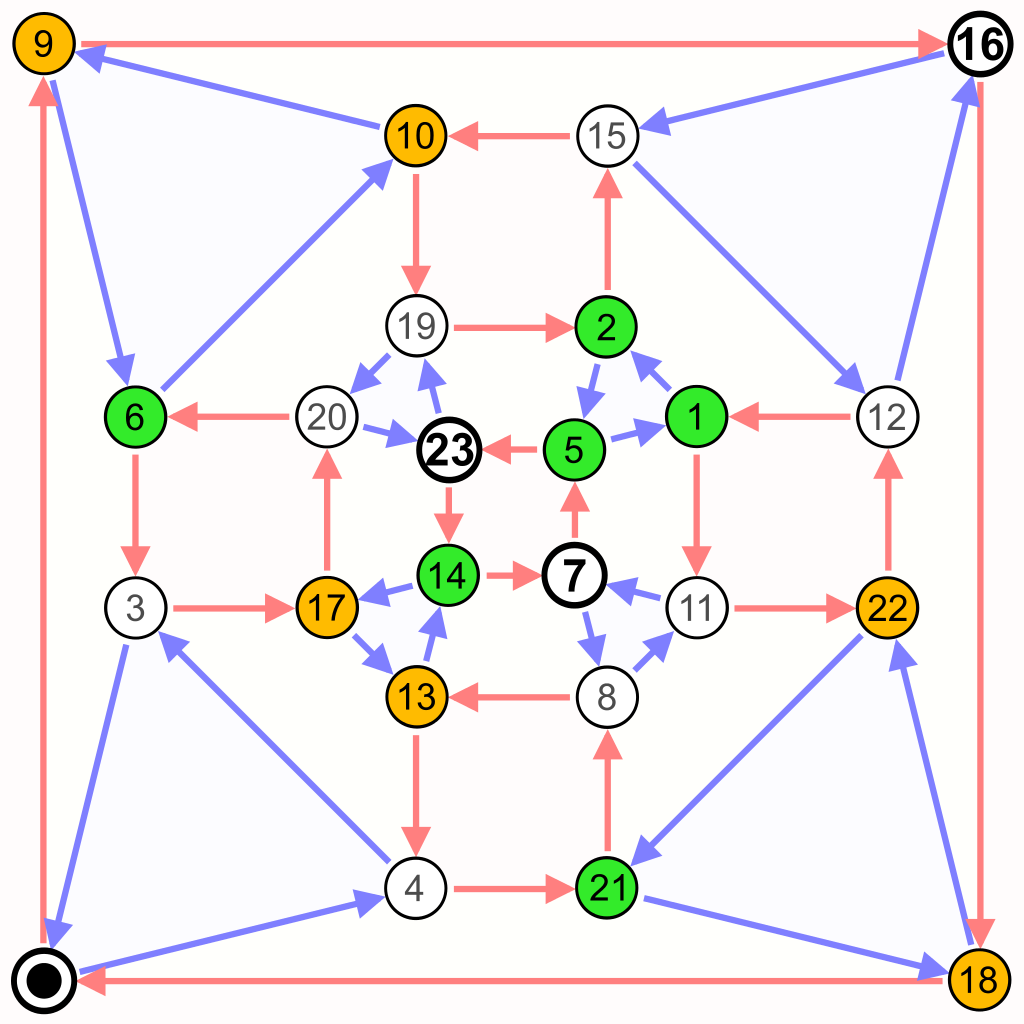
\includegraphics[height=7cm]{numbers.png}
      \caption{Cayley有向图}
      \label{fig:Directed-Cayley-graph}
    \end{minipage}\hfill
    \begin{minipage}{0.48\textwidth}
      \centering
      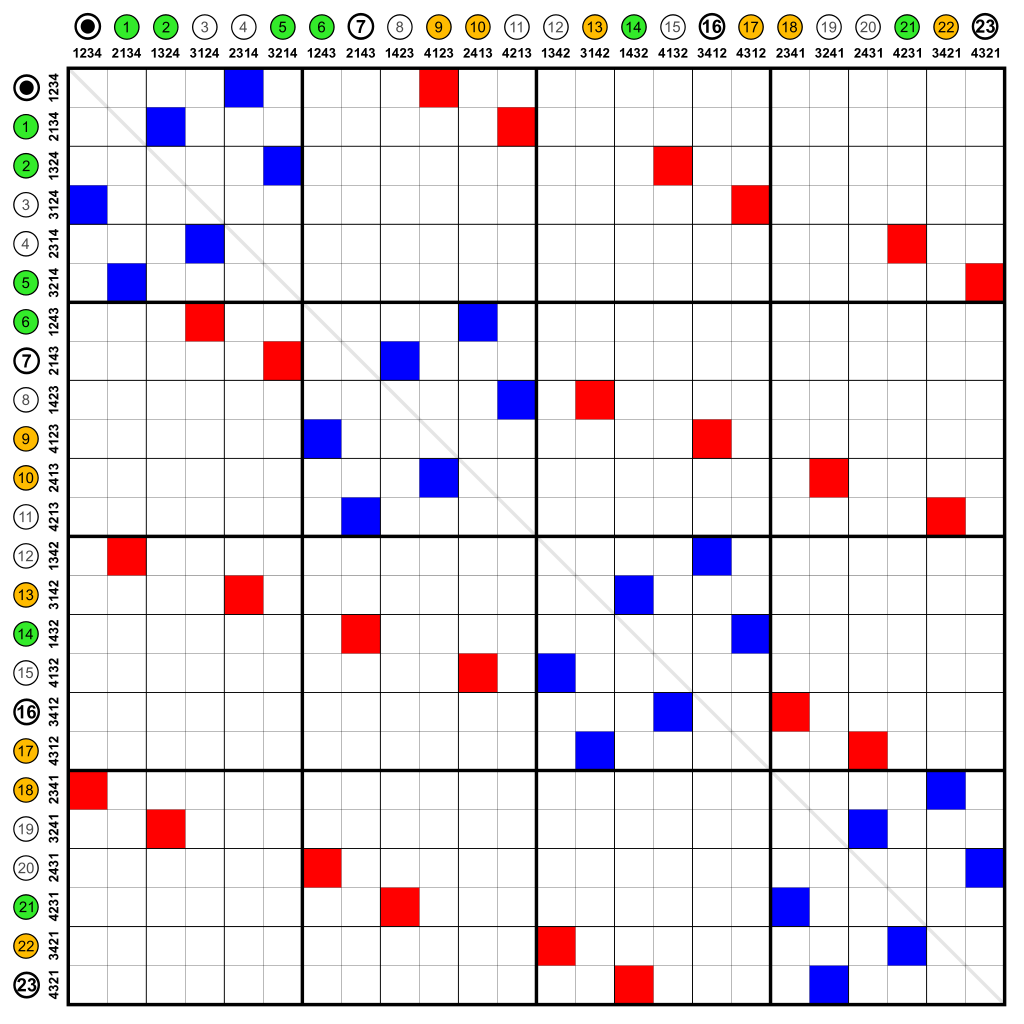
\includegraphics[height=7cm]{adjacency_matrix.png}
      \caption{邻接矩阵}
      \label{fig:Adjacency-matrix}
    \end{minipage}
\end{figure}

\subsection{链式通信协议}
对于一个强连通的电网,我们使用有向图的邻接矩阵A来描述其通信拓扑:

\begin{equation}
    \mathbf{A}=\left[a_{i j}\right]_{N \times N}
\end{equation}

\begin{equation}
    a_{i j}=\left\{\begin{array}{l}
    {1} \\
    {0}
    \end{array}\right.
\end{equation}

其中,1表示通信节点j能向i发送消息并被i接收。

链式通信协议迭代更新每个节点的状态变量如下:

\begin{equation}
    s_{i}^{(k+1)}=\sum_{j=1}^{N} q_{i j} s_{j}^{(k)}, i=1,2, \ldots, N
\end{equation}

矩阵形式为:

\begin{equation}
    \mathbf{s}^{(k+1)}=\mathbf{Q} \mathbf{s}^{(k)}
\end{equation}

由于在电网中,下一轮迭代的状态变量仅和上一轮迭代的状态变量相关,具有无记忆性。参考Markov chain可得,Q为过渡矩阵,有每一次迭代时有向图的边的权重信息。

在实际物理层中,我们选取状态变量为

\begin{equation}
    s_{i}^{(k)}=p_{i}^{(k)}-\alpha_{i}
\end{equation}

其中,$p_{i}^{(k)}$是第k轮迭代的机组i的出力,$\alpha_{i}$为线性外推得到的零边际成本下的假想机组出力。 $s_{i}^{(k)}$是机组i的溢价出力量,这部分出力将抬高机组的边际成本$\lambda_{i}$。

链式通信协议物理含义为:每一回合,每台机组将自身出力按特定比例转移给相邻节点。

\section{过渡矩阵优化}

由Perron–Frobenius定理可知:过渡矩阵的次大特征值$\sigma_{2}$决定链式通信协议收敛速率,主特征向量$\sigma_{1}$(Perron向量)决定链式通信协议的最终收敛结果。因此引入F-范数$\|\mathbf{Q}\|_{F}$优化过渡矩阵,实现机组出力的合理分配,提高收敛速度。

\subsection{F-范数调整过渡矩阵Q的元素值}

使用特定的矩阵范数(matrix norm,模)来简化之后的迭代运算,这里采用弗罗贝尼乌斯范数(Frobenius norm)或称希尔伯特-施密特范数(Hilbert–Schmidt norm),这个范数可用不同的方式定义:

\begin{equation}
    \|A\|_{F}=\sqrt{\sum_{i=1}^{m} \sum_{j=1}^{n}\left|a_{i j}\right|^{2}}=\sqrt{\operatorname{trace}\left(A^{*} A\right)}=\sqrt{\sum_{i=1}^{\min \{m, n\}} \sigma_{i}^{2}}
\end{equation}

这里A*表示A的共轭转置,σi是A的奇异值(特征值),并使用了迹函数。弗罗贝尼乌斯范数与Kn上欧几里得范数非常类似,来自所有矩阵的空间上一个内积。

弗罗贝尼乌斯范数是服从乘法的且在数值线性代数中非常有用。这个范数通常比诱导范数容易计算。

在这里有:

\begin{equation}
    \|\mathbf{Q}\|_{F}=\sqrt{\sum_{i=1}^{N} \sum_{i=1}^{N}\left|q_{i j}\right|^{2}}
\end{equation}

\begin{equation}
    \|\mathbf{Q}\|_{F} \geq \sqrt{\sum_{i=1}^{N}\left|\sigma_{i}\right|^{2}}
\end{equation}

\begin{equation}
    1=\left|\sigma_{1}\right| \geq\left|\sigma_{2}\right| \geq \ldots \geq\left|\sigma_{N}\right|
\end{equation}

优化目标函数:

\begin{equation}
    \min \|\mathbf{Q}\|_{F}^{2}=\sum_{i=1}^{N} \sum_{i=1}^{N}\left|q_{i j}\right|
\end{equation}

优化目标函数物理意义:最小化F范数,相当于最小化次大特征值,优化收敛速率

\subsection{过渡矩阵Q的约束}

过渡矩阵Q满足以下约束条件:

\begin{equation}
    \mathbf{Q}=\left[q_{i j}\right]_{N \times N}
\end{equation}

\begin{equation}
    q_{i j}\left\{\begin{array}{l}
    {\geq 0} \\
    {=0}
    \end{array}\right.
\end{equation}

当节点j不能向节点i发送信息时为0

还需要保证总出力不变:

\begin{equation}
    \mathbf{1}^{T} \mathbf{Q}=\mathbf{1}^{T}
\end{equation}

即:

\begin{equation}
    \sum_{j=1}^{N} q_{i j} \beta_{j}=\beta_{i}, i=1,2, \ldots, N
\end{equation}

为使得链式通信协议收敛于过渡矩阵Q,需保证过渡矩阵的Perron向量恰好等于出力-价格灵敏度向量$\boldsymbol{\beta}=\left[\beta_{1}, \beta_{2}, \ldots, \beta_{N}\right]^{T}$,即保证出力比稳定为$\boldsymbol{\beta}_{1}: \boldsymbol{\beta}_{2} \ldots$。其中$\lambda_{i}=p_{i} / \beta_{i}$,即机组i的成本微增率与出力成正比,$\boldsymbol{\beta}$为出力/价格比例系数。

\begin{equation}
    \mathbf{Q} \boldsymbol{\beta}=\boldsymbol{\beta}
\end{equation}

即:

\begin{equation}
    \sum_{j=1}^{N} q_{i j} \beta_{j}=\beta_{i}, i=1,2, \ldots, N
\end{equation}

\subsection{过渡矩阵优化求解}

即求解以下二次规划问题:

\begin{equation}
    \begin{aligned}
    &\min _{q_{y}}\|\mathbf{Q}\|_{F}^{2}=\sum_{i=1}^{N} \sum_{i=1}^{N}\left|q_{i j}\right|^{2}\\
    &\text { s.t. } \quad q_{i j}\left\{\begin{array}{ll}
    {\geq 0} & {\quad a_{i j}=1} \\
    {=0} & {\quad a_{i j}=0}
    \end{array}\right.\\
    &\mathbf{1}^{T} \mathbf{Q}=\mathbf{1}^{T}\\
    &\mathbf{Q} \boldsymbol{\beta}=\boldsymbol{\beta}
    \end{aligned}
\end{equation}

一般二次规划问题求解形式为:

\begin{equation}
    \begin{aligned}
    &\min \mathbf{x}^{T} \mathbf{x}\\
    &\text { s.t. } \quad \mathbf{A}_{1} \mathbf{x}=\mathbf{b}_{1}
    \end{aligned}
\end{equation}

其中x的每一个元素即是过渡矩阵Q的一个非零元素。该二次规划问题的优化解为:

\begin{equation}
    \mathbf{x}^{*}=\mathbf{A}_{1}^{T}\left(\mathbf{A}_{1} \mathbf{A}_{1}^{T}\right)^{-1} \mathbf{b}_{1}
\end{equation}

将x*的每个元素的值还原到过渡矩阵Q的相应位置上,可得到经优化的过渡阵。

\section{分布式ED协议的实现方式}

每个节点独立算出$\beta_{i}$出力/价格比例系数,

出力-价格灵敏度向量$\boldsymbol{\beta}$与邻接矩阵$\boldsymbol{A}$结合,得出优化后的过渡矩阵$\boldsymbol{Q}$

根据过渡矩阵与链式通信拓扑有向图权重的对应关系,的第j列元素代表始端节点与机组j的边的权重。因此把过渡矩阵$\boldsymbol{Q}$按列拆分,将第j列元素发送给机组j的节点。

节点i独立算出其初始溢价出力量$s_{i}^{(0)}=L_{i}-\alpha_{i}$

按过渡矩阵Q,迭代运行链式通信协议。

\begin{equation}
    s_{i}^{(k+1)}=\sum_{j=1}^{N} q_{i j} s_{j}^{(k)}, i=1,2, \ldots, N
\end{equation}

节点j计算出$q_{i j} s_{j}^{(k)}, i=1,2, \ldots, N$,并分别将$q_{i j} s_{j}^{(k)}$发给节点i。(若$A_{i j}$为0,则此项为0,不影响其他节点)

k次迭代后,节点i的出力和电价为:

\begin{equation}
    \begin{aligned}
    &p_{i}^{(k)}=s_{i}^{(k)}+\alpha_{i}\\
    &\lambda_{i}^{(k)}=s_{i}^{(k)} / \beta_{i}
    \end{aligned}
\end{equation}

当迭代过程中式~\ref{eq:delta}条件满足,则价格达成共识,可以执行目前的定价。

\begin{equation}
    \left|\lambda_{i}^{(k+1)}-\lambda_{i}^{(k)}\right|<\delta
    \label{eq:delta}    
\end{equation}

其中$\delta$为误差容限,表示电价求解精度。

\section{迭代结束将得到帕雷托最优的证明}

本节证明迭代结束时各节点出力达到帕雷托最优(Pareto Optimality),即在误差允许的范围内ED最优解。

\begin{equation}
    \mathbf{1}^{T} \mathbf{s}^{(k+1)}=\mathbf{1}^{T} \mathbf{Q} \mathbf{s}^{(k)}=\mathbf{1}^{T} \mathbf{s}^{(k)}=\mathbf{1}^{T} \mathbf{s}^{(0)}=\sum_{i=1}^{N}\left(L_{i}-\alpha_{i}\right)
\end{equation}

由于终止时各变量趋于稳定,由Perron-由Perron–Frobenius定理:

\begin{equation}
    \mathbf{s}^{(k)}=r \boldsymbol{\beta}
\end{equation}

得:

\begin{equation}
    r=\sum_{i=1}^{N}\left(L_{i}-\alpha_{i}\right) / \sum_{i=1}^{N} \beta_{i}=\lambda_{i}^{(k)}
\end{equation}

表明达到价格共识,并满足功率平衡约束:

\begin{equation}
    \sum_{i=1}^{N}\left(\beta_{i} \lambda_{i}^{(k)}+\alpha_{i}\right)=\sum_{i=1}^{N} L_{i}
\end{equation}

\section{考虑每个节点出力上下限的处理}

当某节点的出力超上下限时,可用虚拟功率法调整出力分配。

\begin{equation}
    S_{i}^{(k+1)}=\left(\sum_{j=1}^{n} q_{i j}\left(s_{j}^{(k)}+\Delta p_{j}^{(k)}\right)\right)-\Delta p_{i}^{(k)}
\end{equation}

\begin{equation}
    \Delta p_{i}^{(k+1)}=\max \left\{\Delta p_{i}^{(k)}+r_{i}^{(k)}\left(s_{i}^{(k)}+\alpha-\bar{p}_{i}\right), 0\right\}
\end{equation}

k能被t整除时为1,反之为0:

\begin{equation}
    r_{i}^{(k)}=\left\{\begin{array}{l}
    {1} \\
    {0}
    \end{array}\right.
\end{equation}


终止条件增加一条:$\Delta p_{i}^{(k)}=0$

$\Delta p_{i}^{(k)}$为机组i引进的虚拟功率,取值为非负数。当机组i的出力到达上限时,由于向外发送了出力,导致整个系统价格抬高。


\section{算例}

设想一个四节点机组网络有向图如图~\ref{fig:Directed-graph}:

%去除Visio白边:http://www.mamicode.com/info-detail-2181323.html

\begin{figure}[htbp] % use float package if you want it here
    \centering
    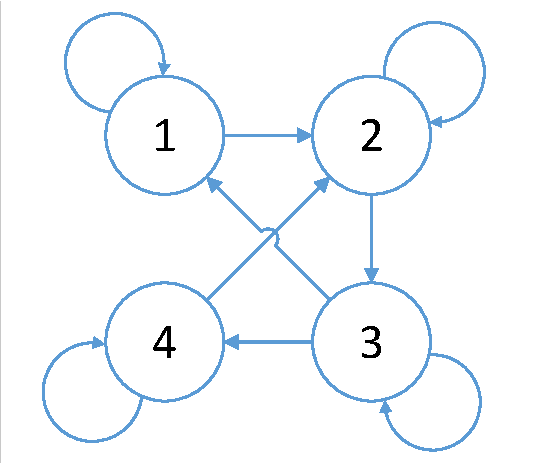
\includegraphics{Directed-graph.pdf}
    \caption{四节点机组网络有向图}
    \label{fig:Directed-graph}
\end{figure}

各节点处机组参数与负荷如表~\ref{tab:example}:

\begin{table}[]
    \centering
%    \resizebox{\textwidth}{!}{%
    \begin{tabular}{@{}ccccc@{}}
    \toprule
    \multicolumn{1}{c}{Node} & $\alpha_{i}(\mathrm{MW})$  & $\beta_{i} \quad\left(\mathrm{MW}^{2} / \mathrm{S}\right)$ & $\gamma_{i}(\mathrm{S})$   & $L_{i}(\mathrm{MW})$    \\ \midrule
    1                        & -1 & 1 & 0.2 & 15.5 \\
    2                        & -2 & 2 & 0.1 & 0    \\
    3                        & -3 & 3 & 0.5 & 15.5 \\
    4                        & -1 & 2 & 0.7 & 0    \\ \bottomrule
    \end{tabular}
%    }缩放表格(字会变得很大)
    \caption{4节点算例机组参数与实时负荷}
    \label{tab:example}
\end{table}

随着迭代各机组的价格曲线如图所示
\chapter{测试平台硬件架构}
\label{cha:Hardware}

\section{平台选型}

我们选用Nvidia Jetson NANO(如图~\ref{fig:Jetson-Nano})作为主要的开发平台,NVIDIA Jetson Nano开发人员工具包是一台功能强大的小型计算机,可并行运行多个神经网络,以用于图像分类,对象检测,分段和语音处理等应用,该平台的功耗仅为5瓦。

\begin{figure}[htbp] % use float package if you want it here
    \centering
    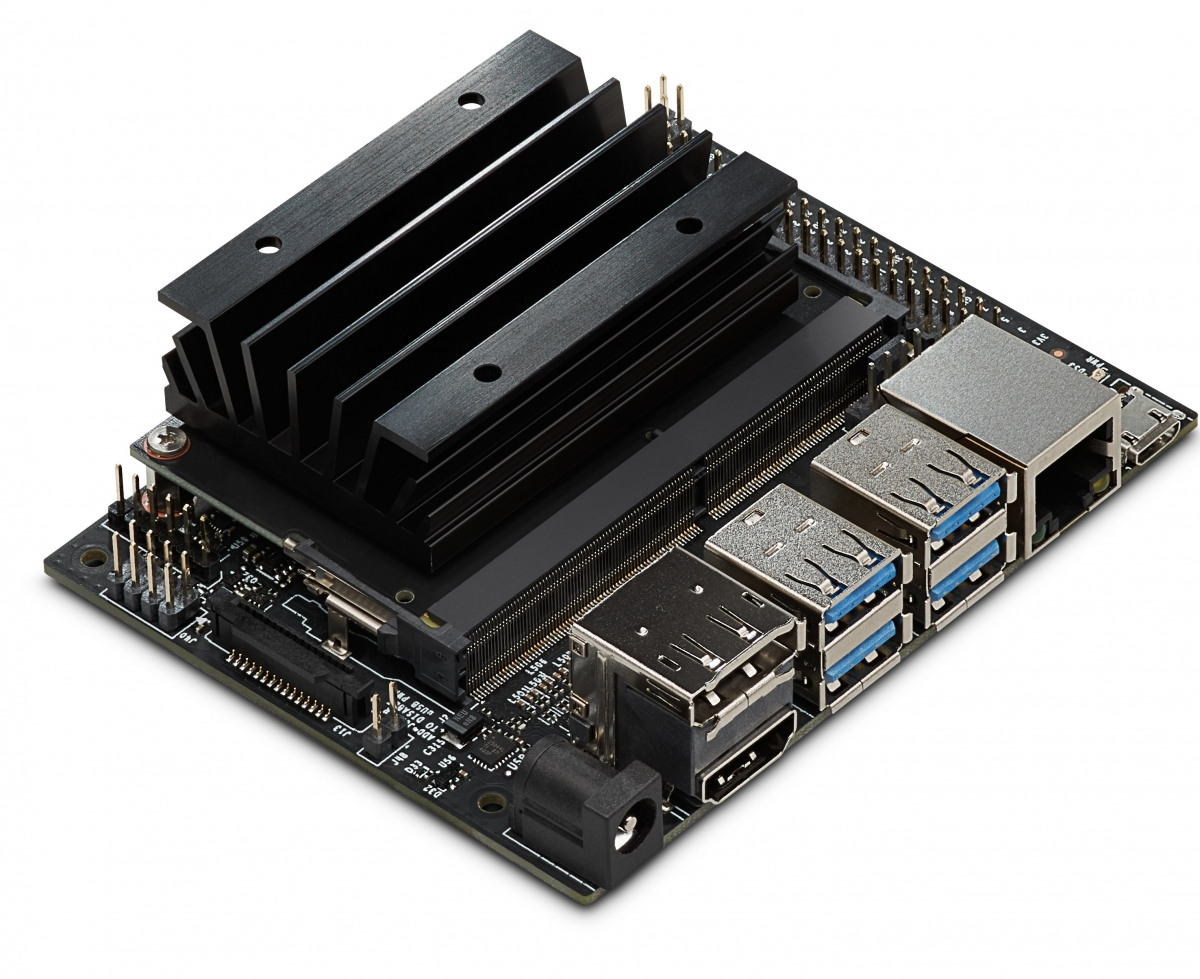
\includegraphics[height=6cm]{Jetson-Nano.jpg}
    \caption{Nvidia Jetson NANO}
    \label{fig:Jetson-Nano}
\end{figure}

初步的硬件平台,采用无线局域网通信,图~\ref{fig:wifi}为将AC8265和片状5GHz天线装到Jetson Nano Developer Kit上。

\begin{figure}[htbp]
    \begin{minipage}{0.48\textwidth}
      \centering
      \includegraphics[height=5cm]{DA4A3052.JPG}
      \caption{为Nano添加无线网功能}
      \label{fig:wifi}
    \end{minipage}\hfill
    \begin{minipage}{0.48\textwidth}
      \centering
      \includegraphics[height=5cm]{DA4A3066.JPG}
      \caption{两机组通信测试平台}
      \label{fig:two-setup}
    \end{minipage}
\end{figure}


\section{电机和全向轮配置}

尝试多种电机与全向轮的配合方式,寻找最优方案:

同样体积的直流减速电机的扭矩比步进电机要大,拥有编码器的电机(如图~\ref{fig:Motor-1})能够反馈实时转速,从而可以使用PID控制进行控制;带有蜗杆的电机(如图~\ref{fig:Motor-2})可以缩小底盘面积,但蜗杆传动使得动力传输方向不可逆,即无法通过转动轮子带动电机转动,这使得手动推动平台变得困难、不顺滑;反折的N20电机(如图~\ref{fig:Motor-3})同样可以缩小底盘面积,但不带编码器的情况下电机尾部就已经和轮子摩擦,在联轴器完全紧固的情况下无法正常工作。

\begin{figure}[htbp]
  \begin{minipage}{0.31\textwidth}
    \centering
    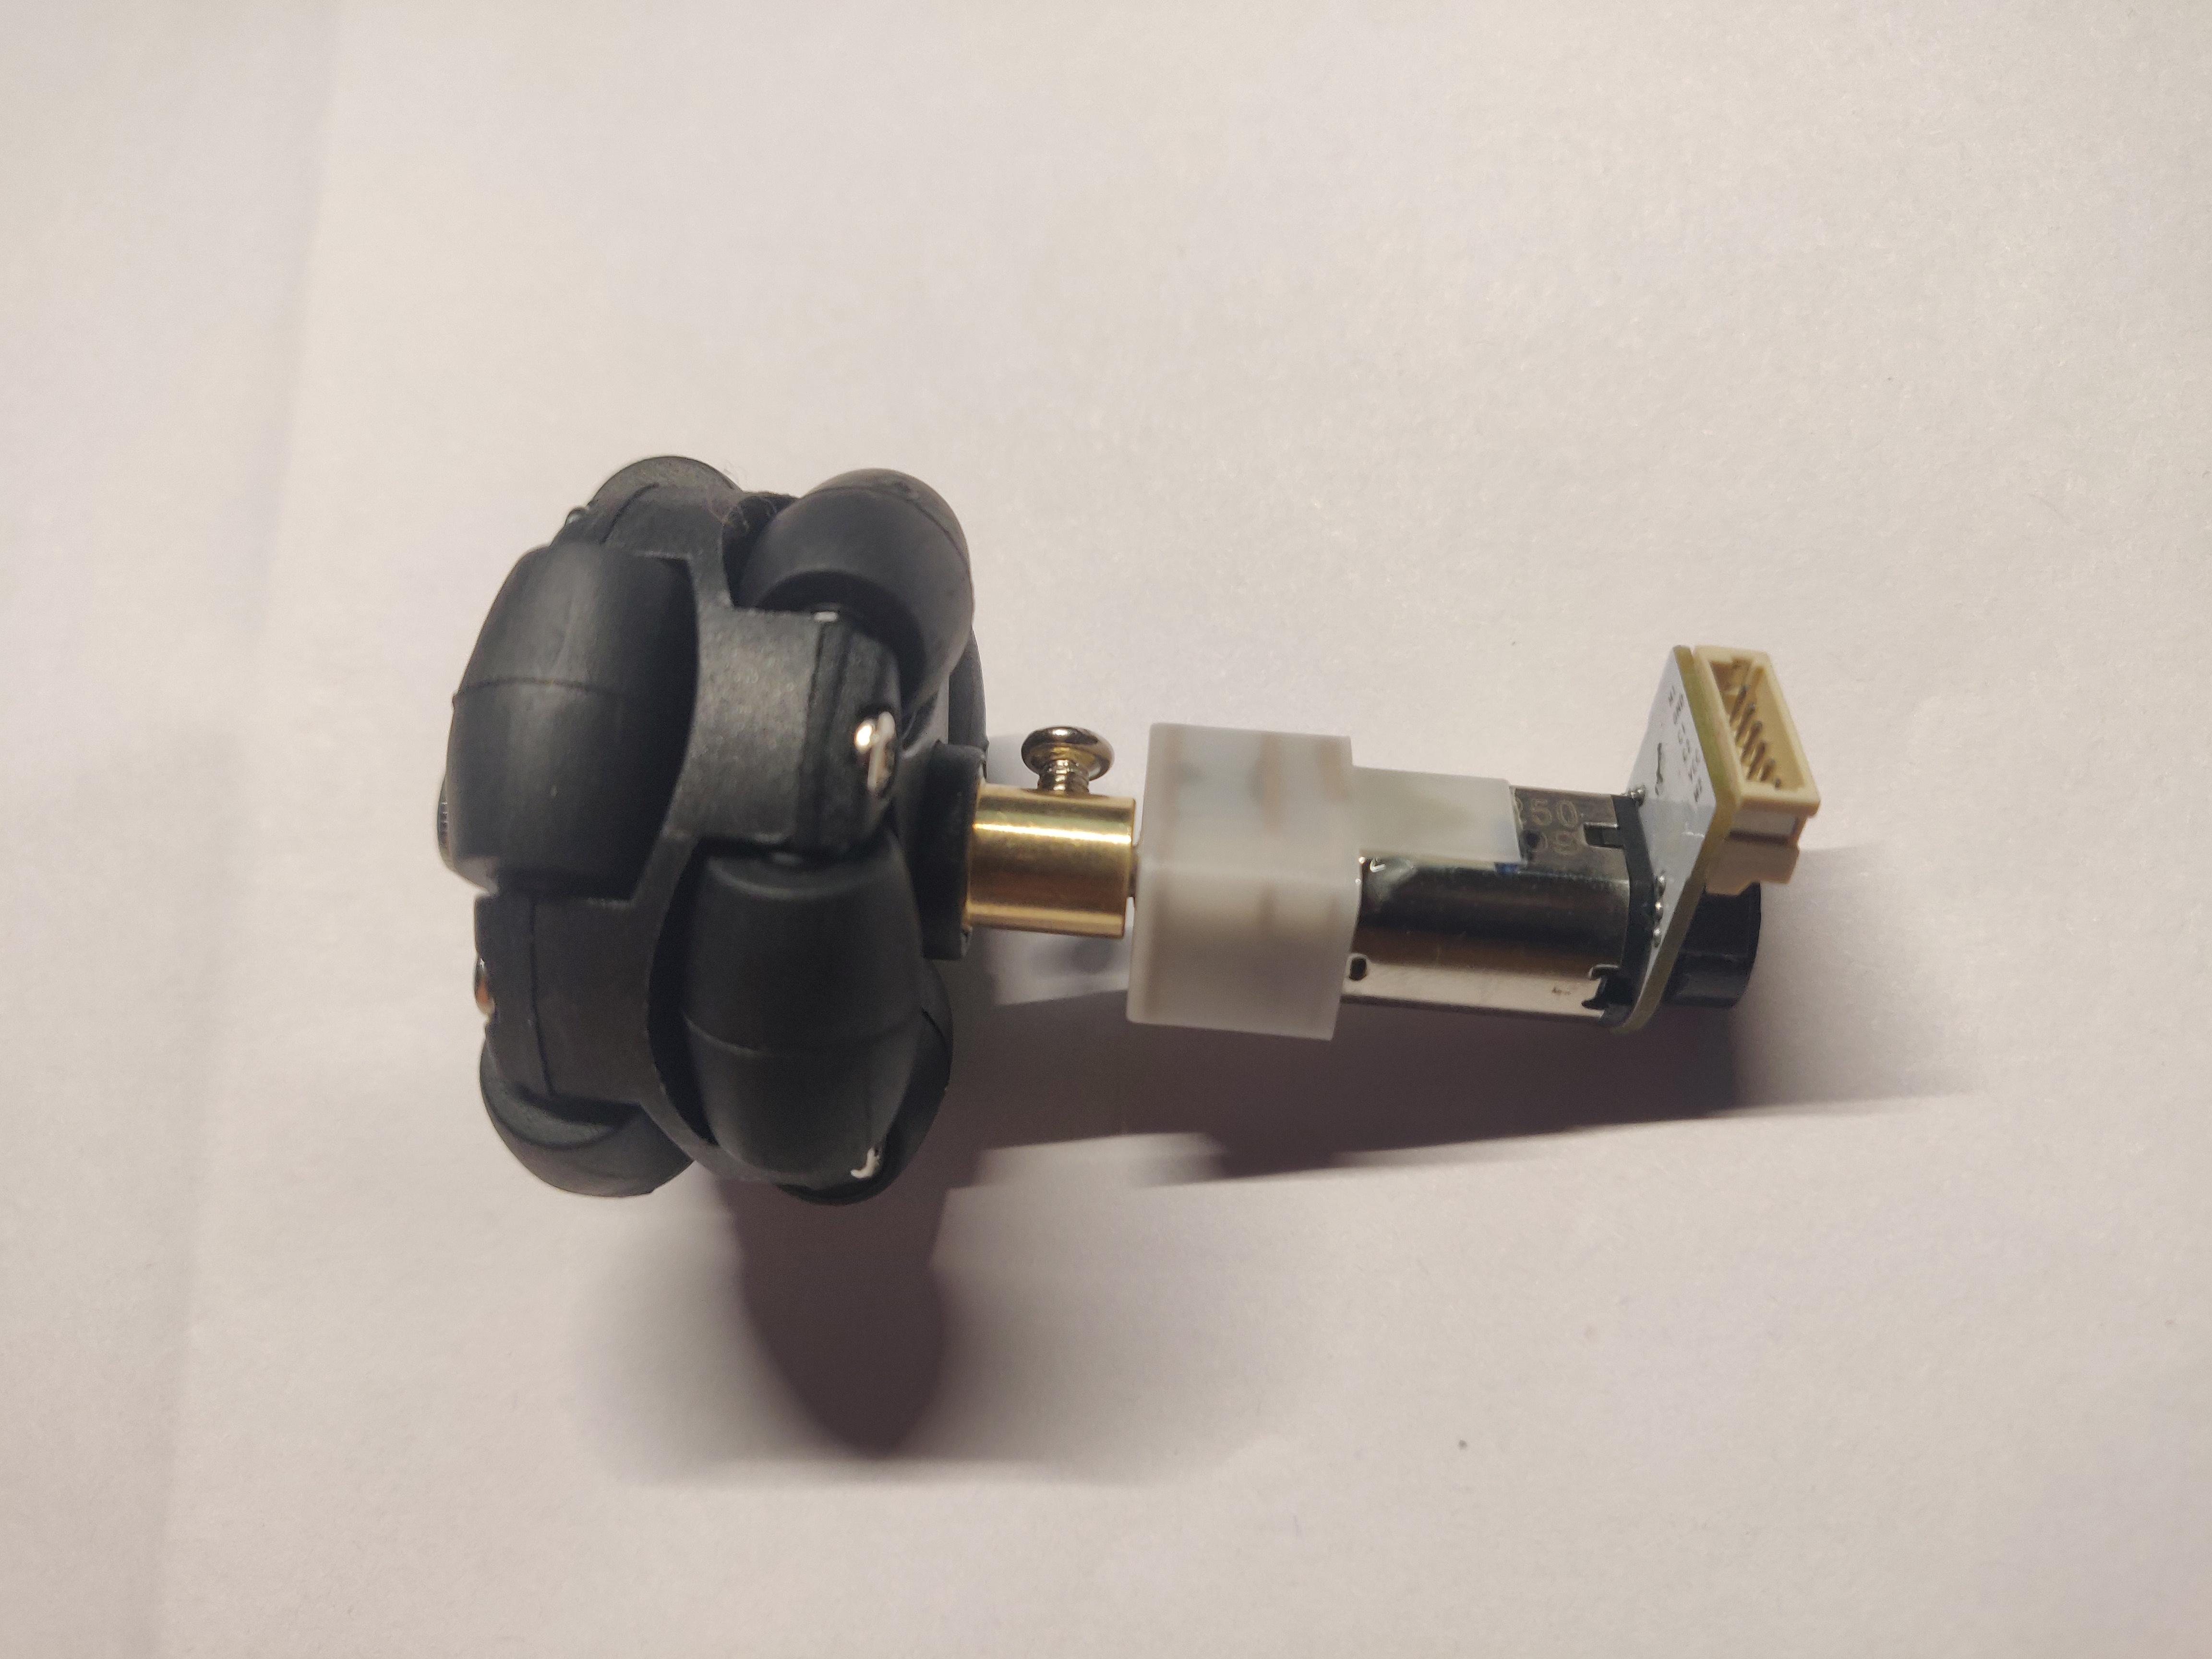
\includegraphics[height=4cm]{Motor-1.jpg}
    \caption{N20减速电机(带编码器)}
    \label{fig:Motor-1}
  \end{minipage}\hfill
  \begin{minipage}{0.31\textwidth}
    \centering
    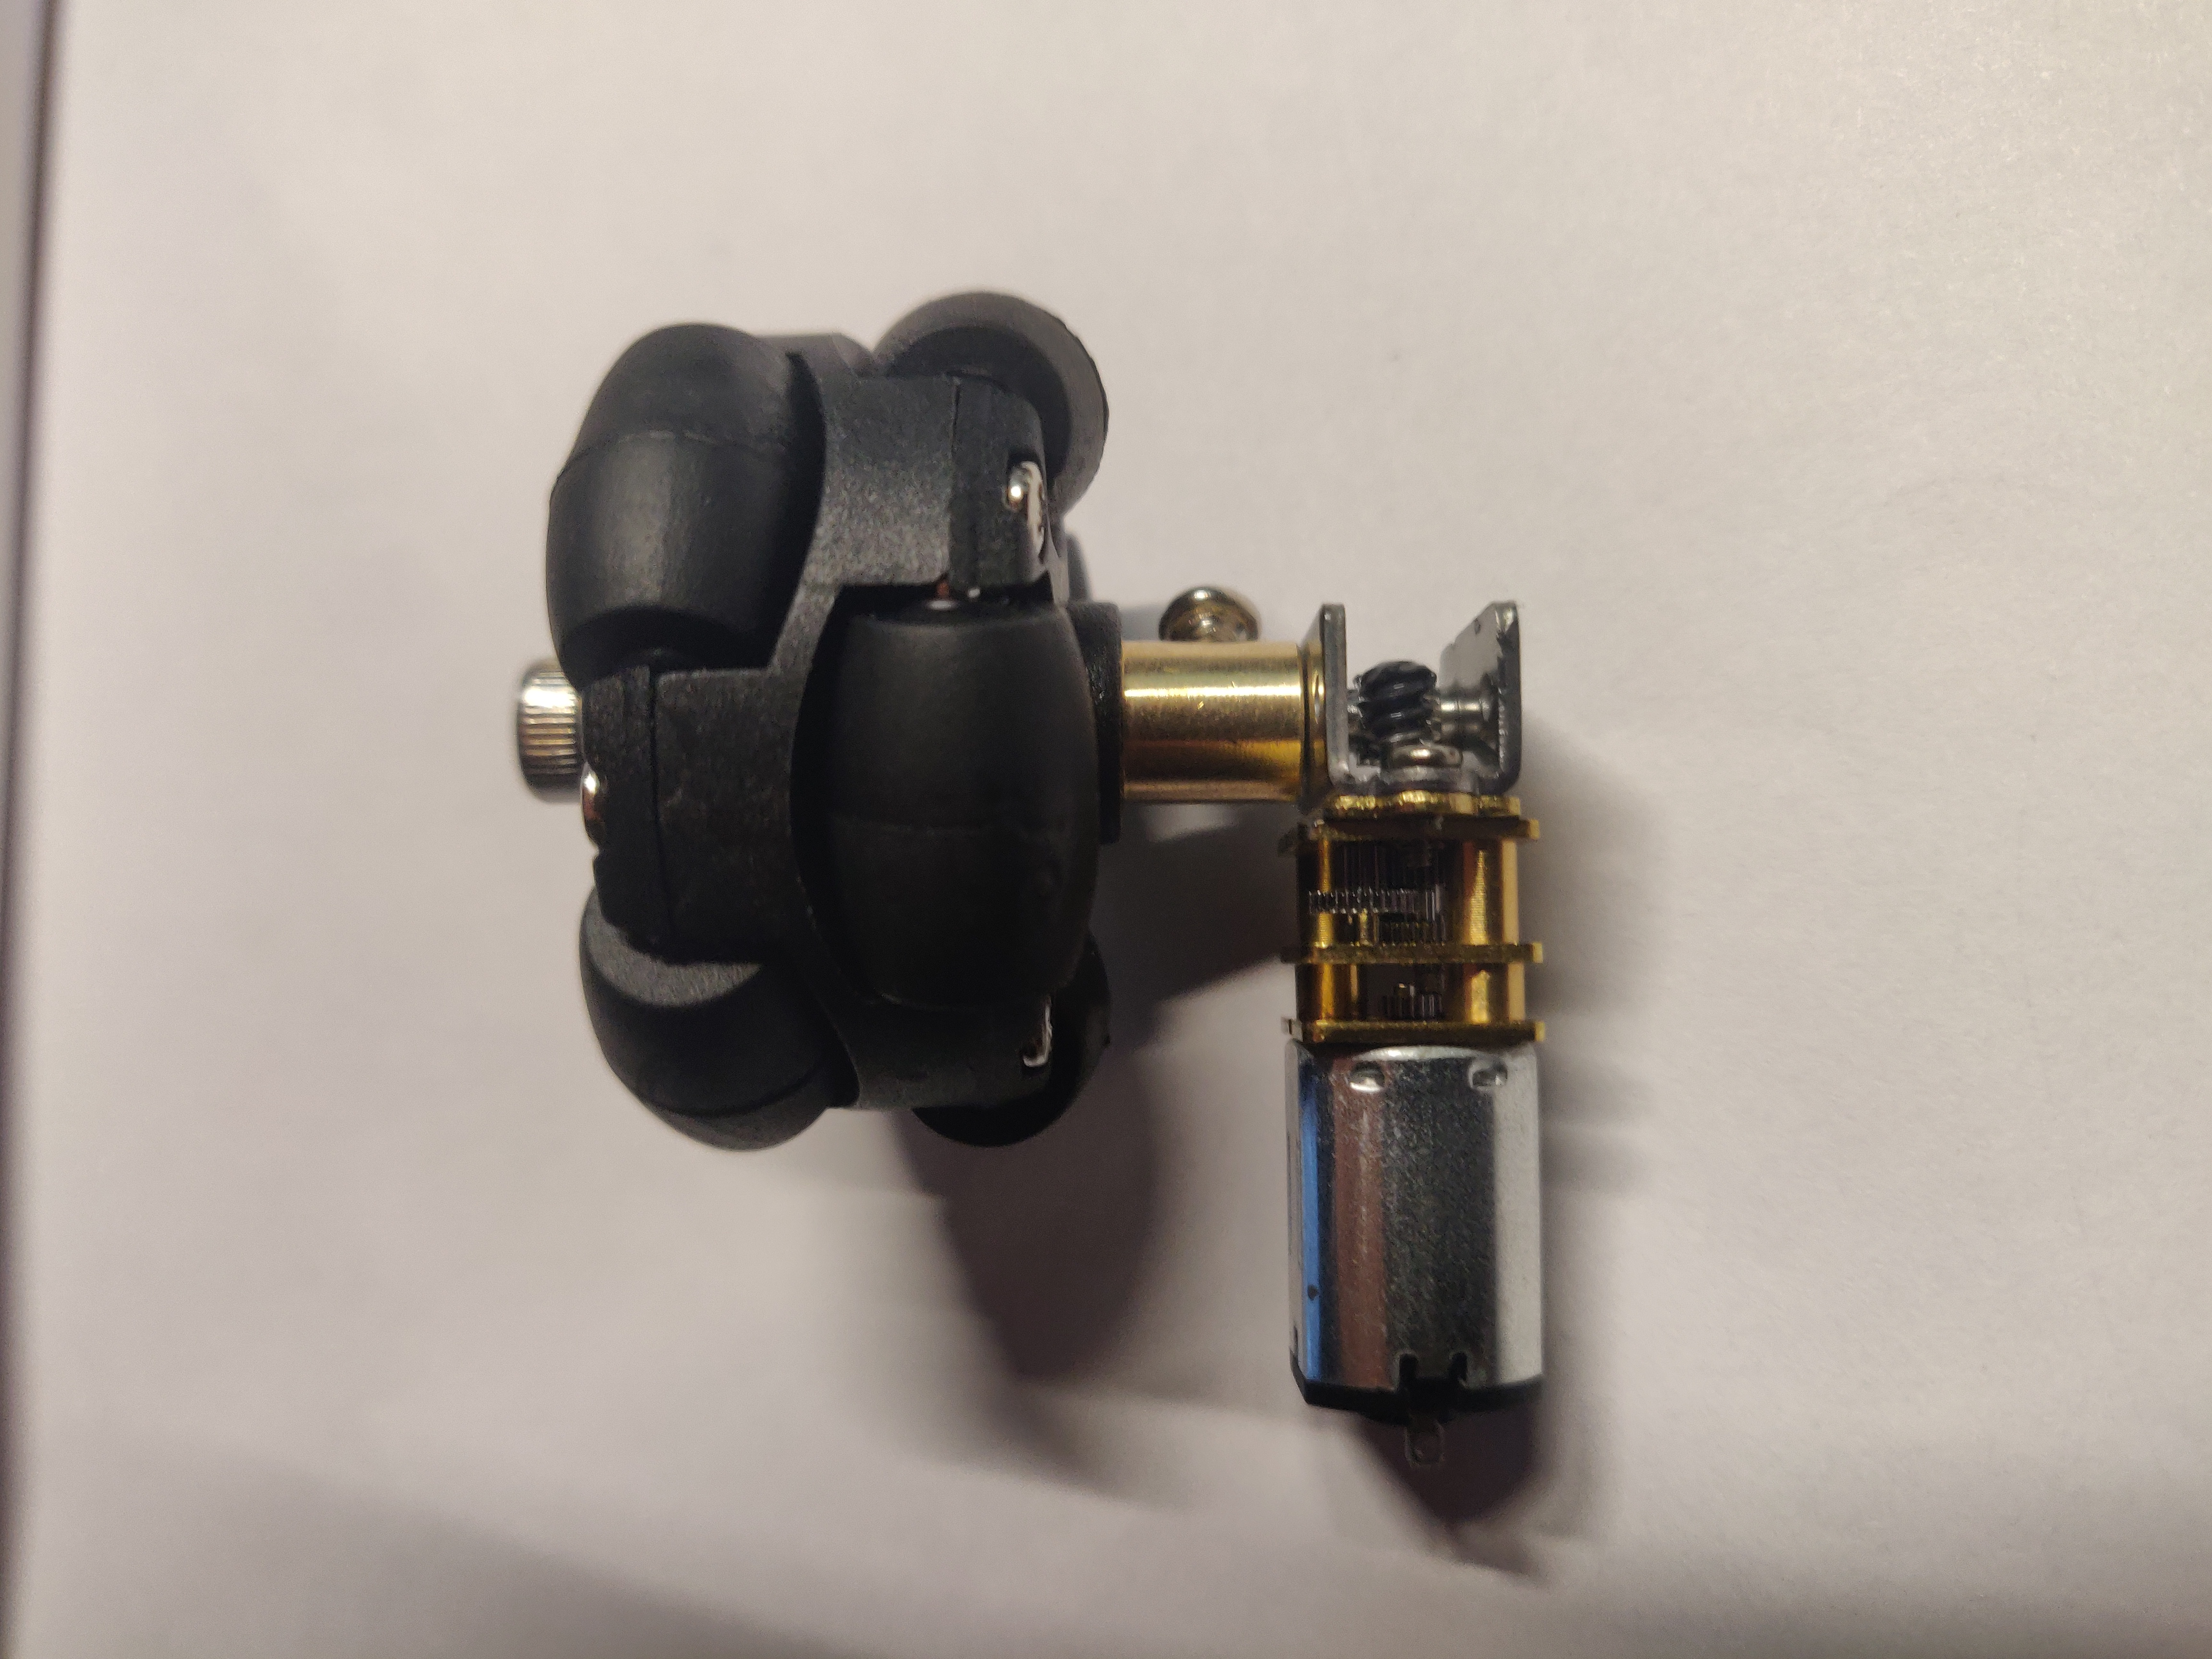
\includegraphics[height=4cm]{Motor-2.jpg}
    \caption{N20减速电机(带蜗杆)}
    \label{fig:Motor-2}
  \end{minipage}\hfill
  \begin{minipage}{0.31\textwidth}
    \centering
    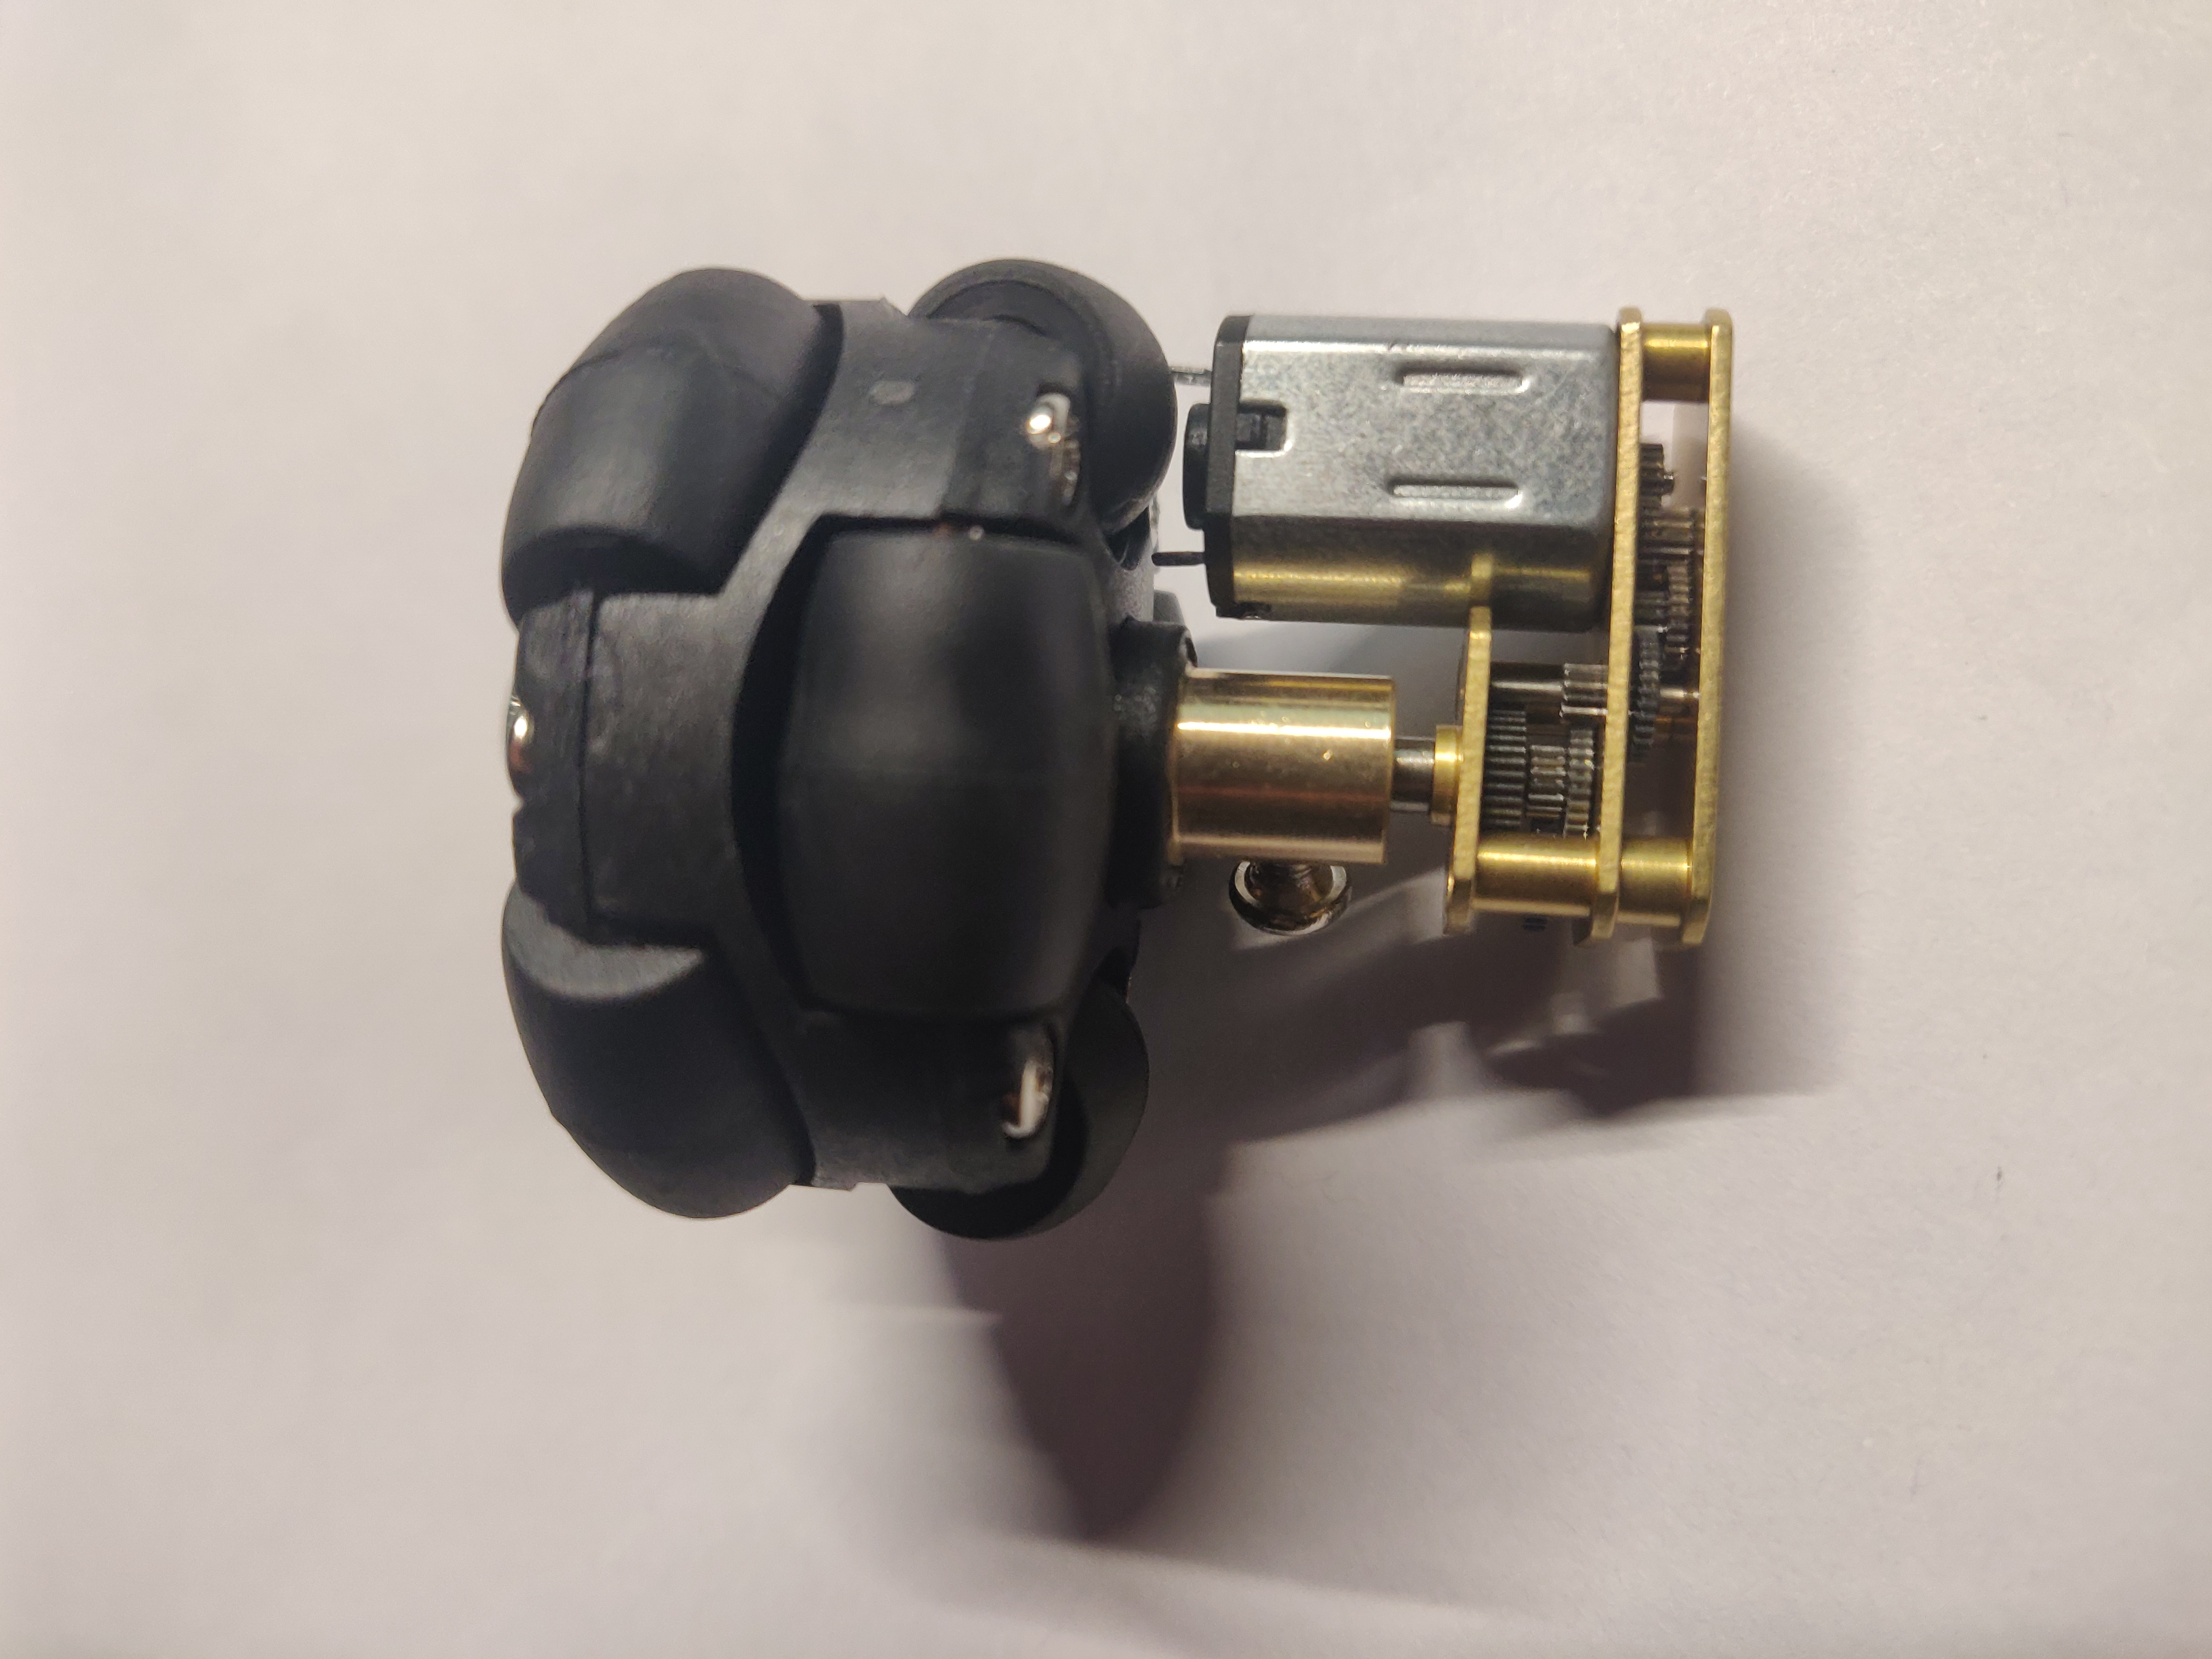
\includegraphics[height=4cm]{Motor-3.jpg}
    \caption{N20减速电机(反折)}
    \label{fig:Motor-3}
  \end{minipage}
\end{figure}

步进电机无需编码器即可控制当前电机的角度,我们考虑体积较小的两相四线微型步进电机:反折的步进电机(如图~\ref{fig:Motor-Step-1})可以缩小底盘面积,另外还有两种不同大小和扭矩的直线步进电机(如图~\ref{fig:Motor-Step-2}和图~\ref{fig:Motor-Step-3})。

\begin{figure}[htbp]
  \begin{minipage}{0.31\textwidth}
    \centering
    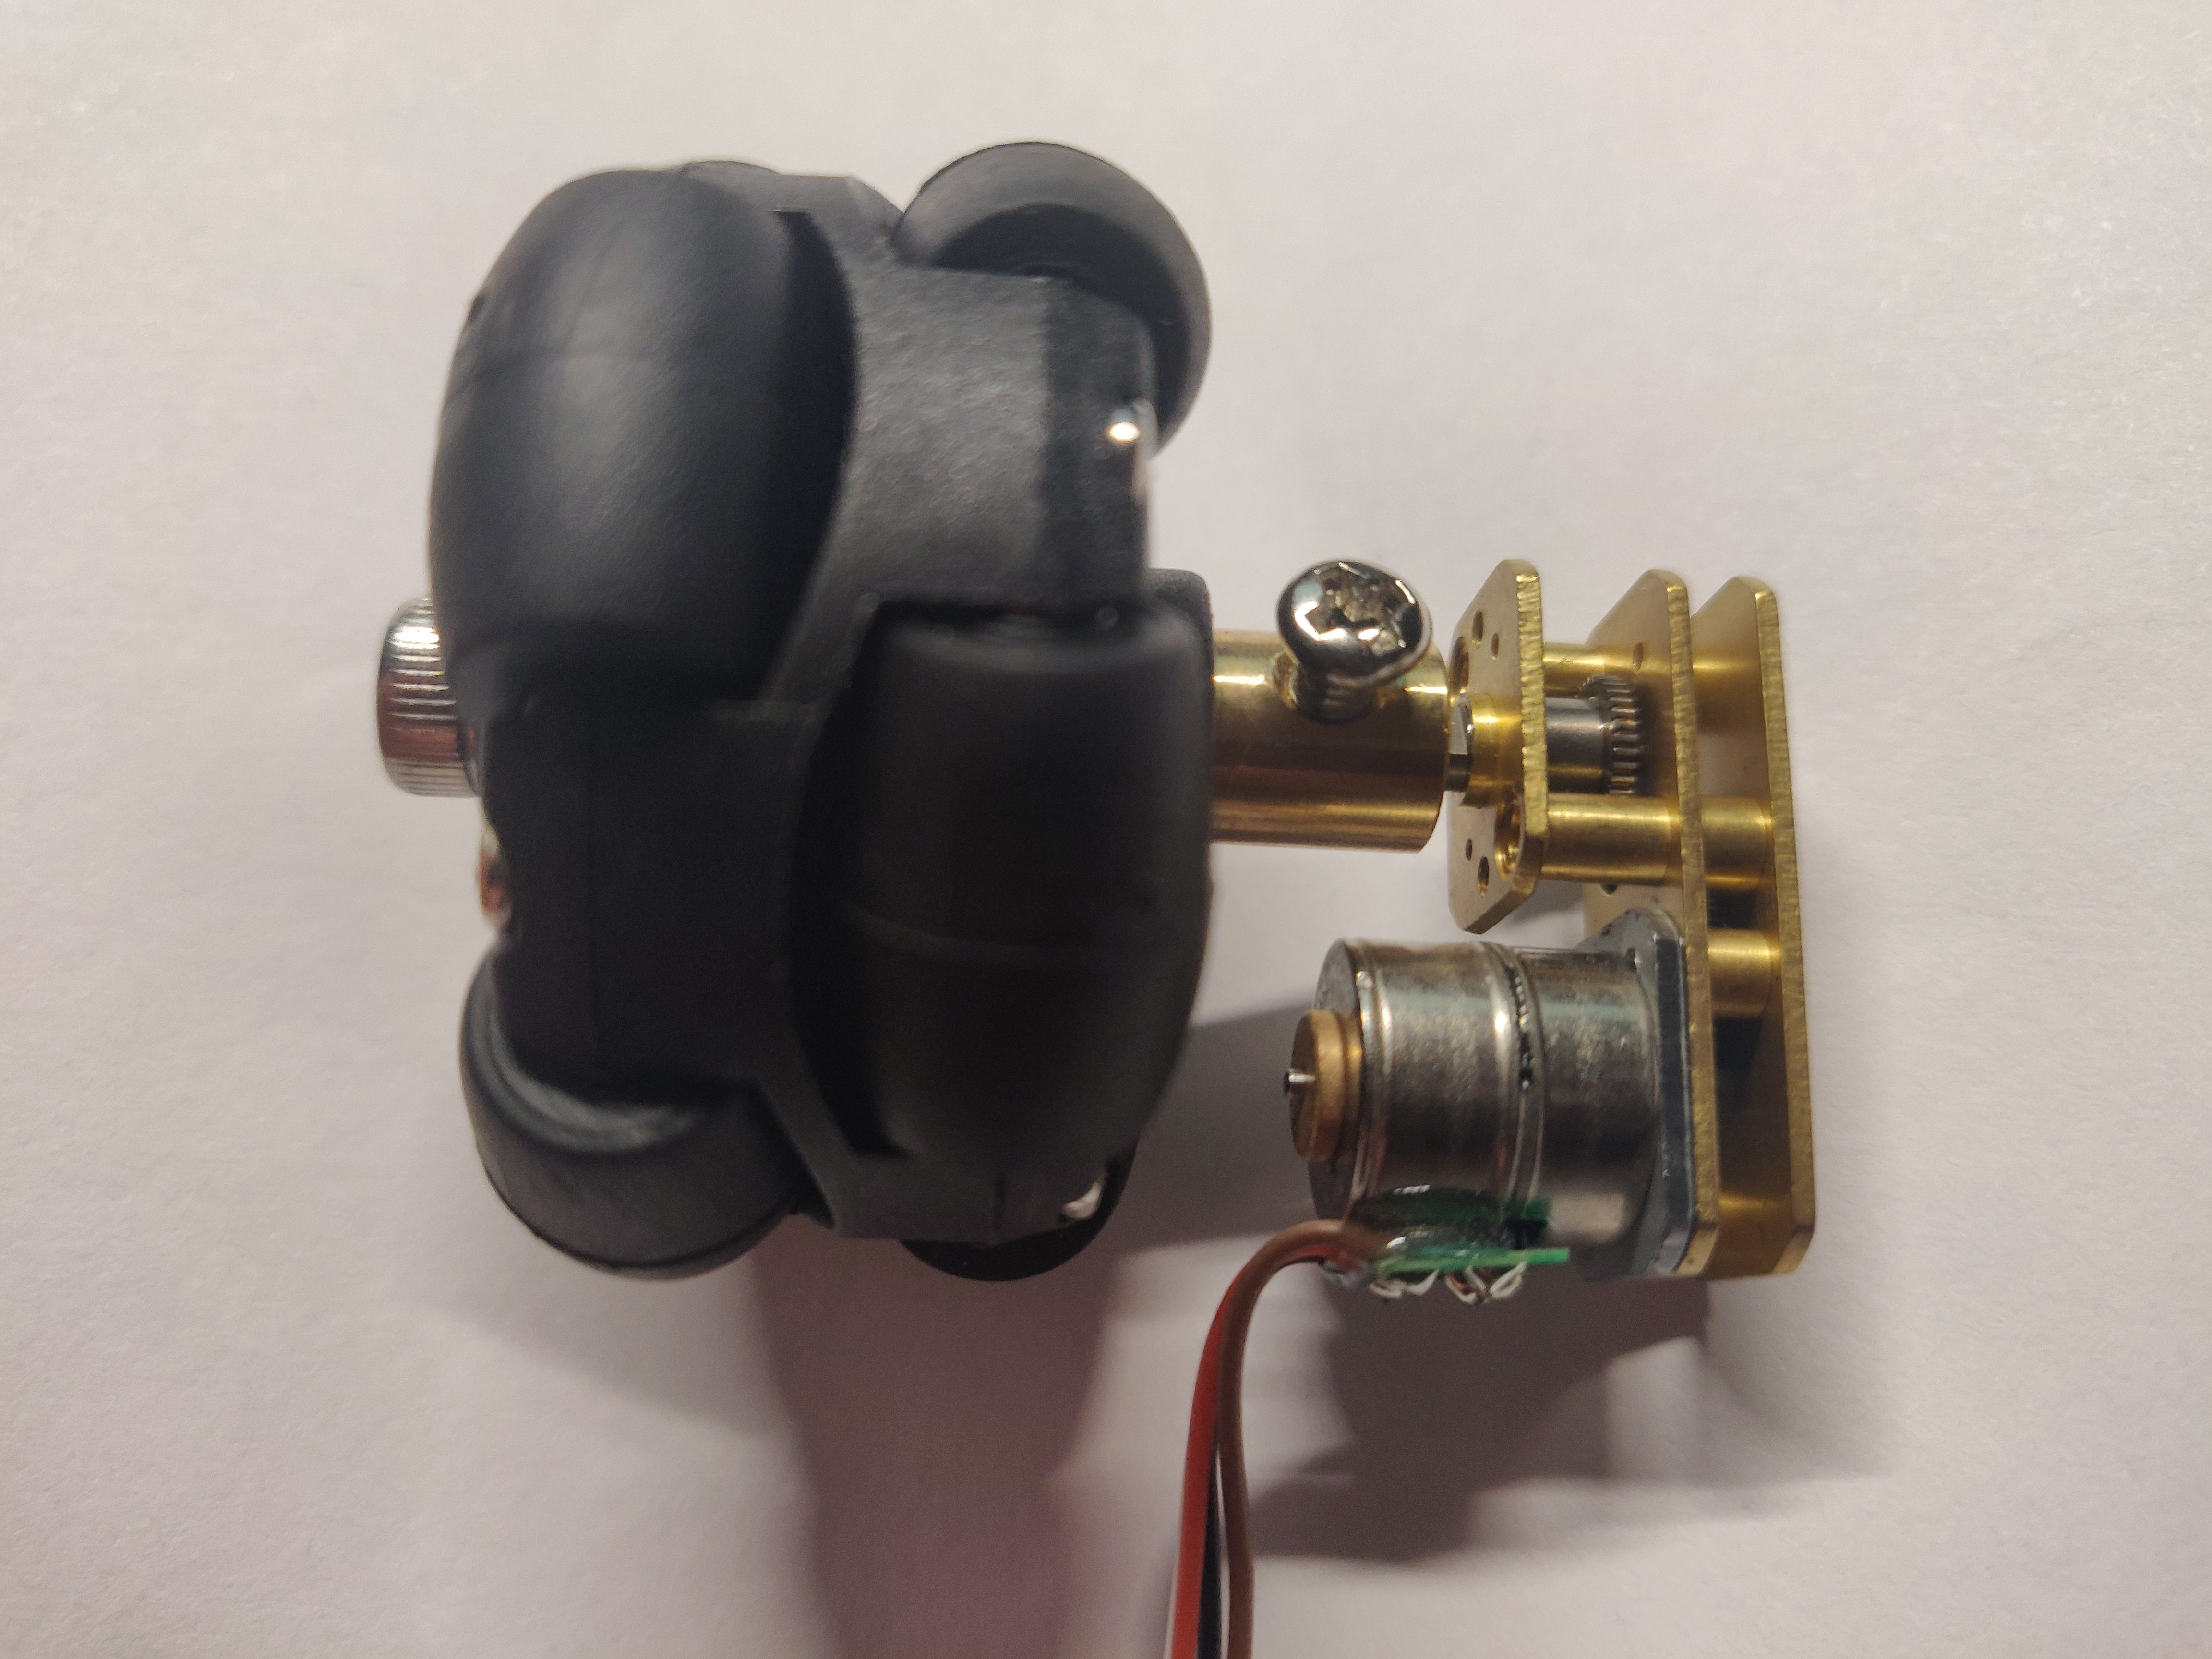
\includegraphics[height=4cm]{Motor-Step-1.jpg}
    \caption{反折的微型步进电机}
    \label{fig:Motor-Step-1}
  \end{minipage}\hfill
  \begin{minipage}{0.31\textwidth}
    \centering
    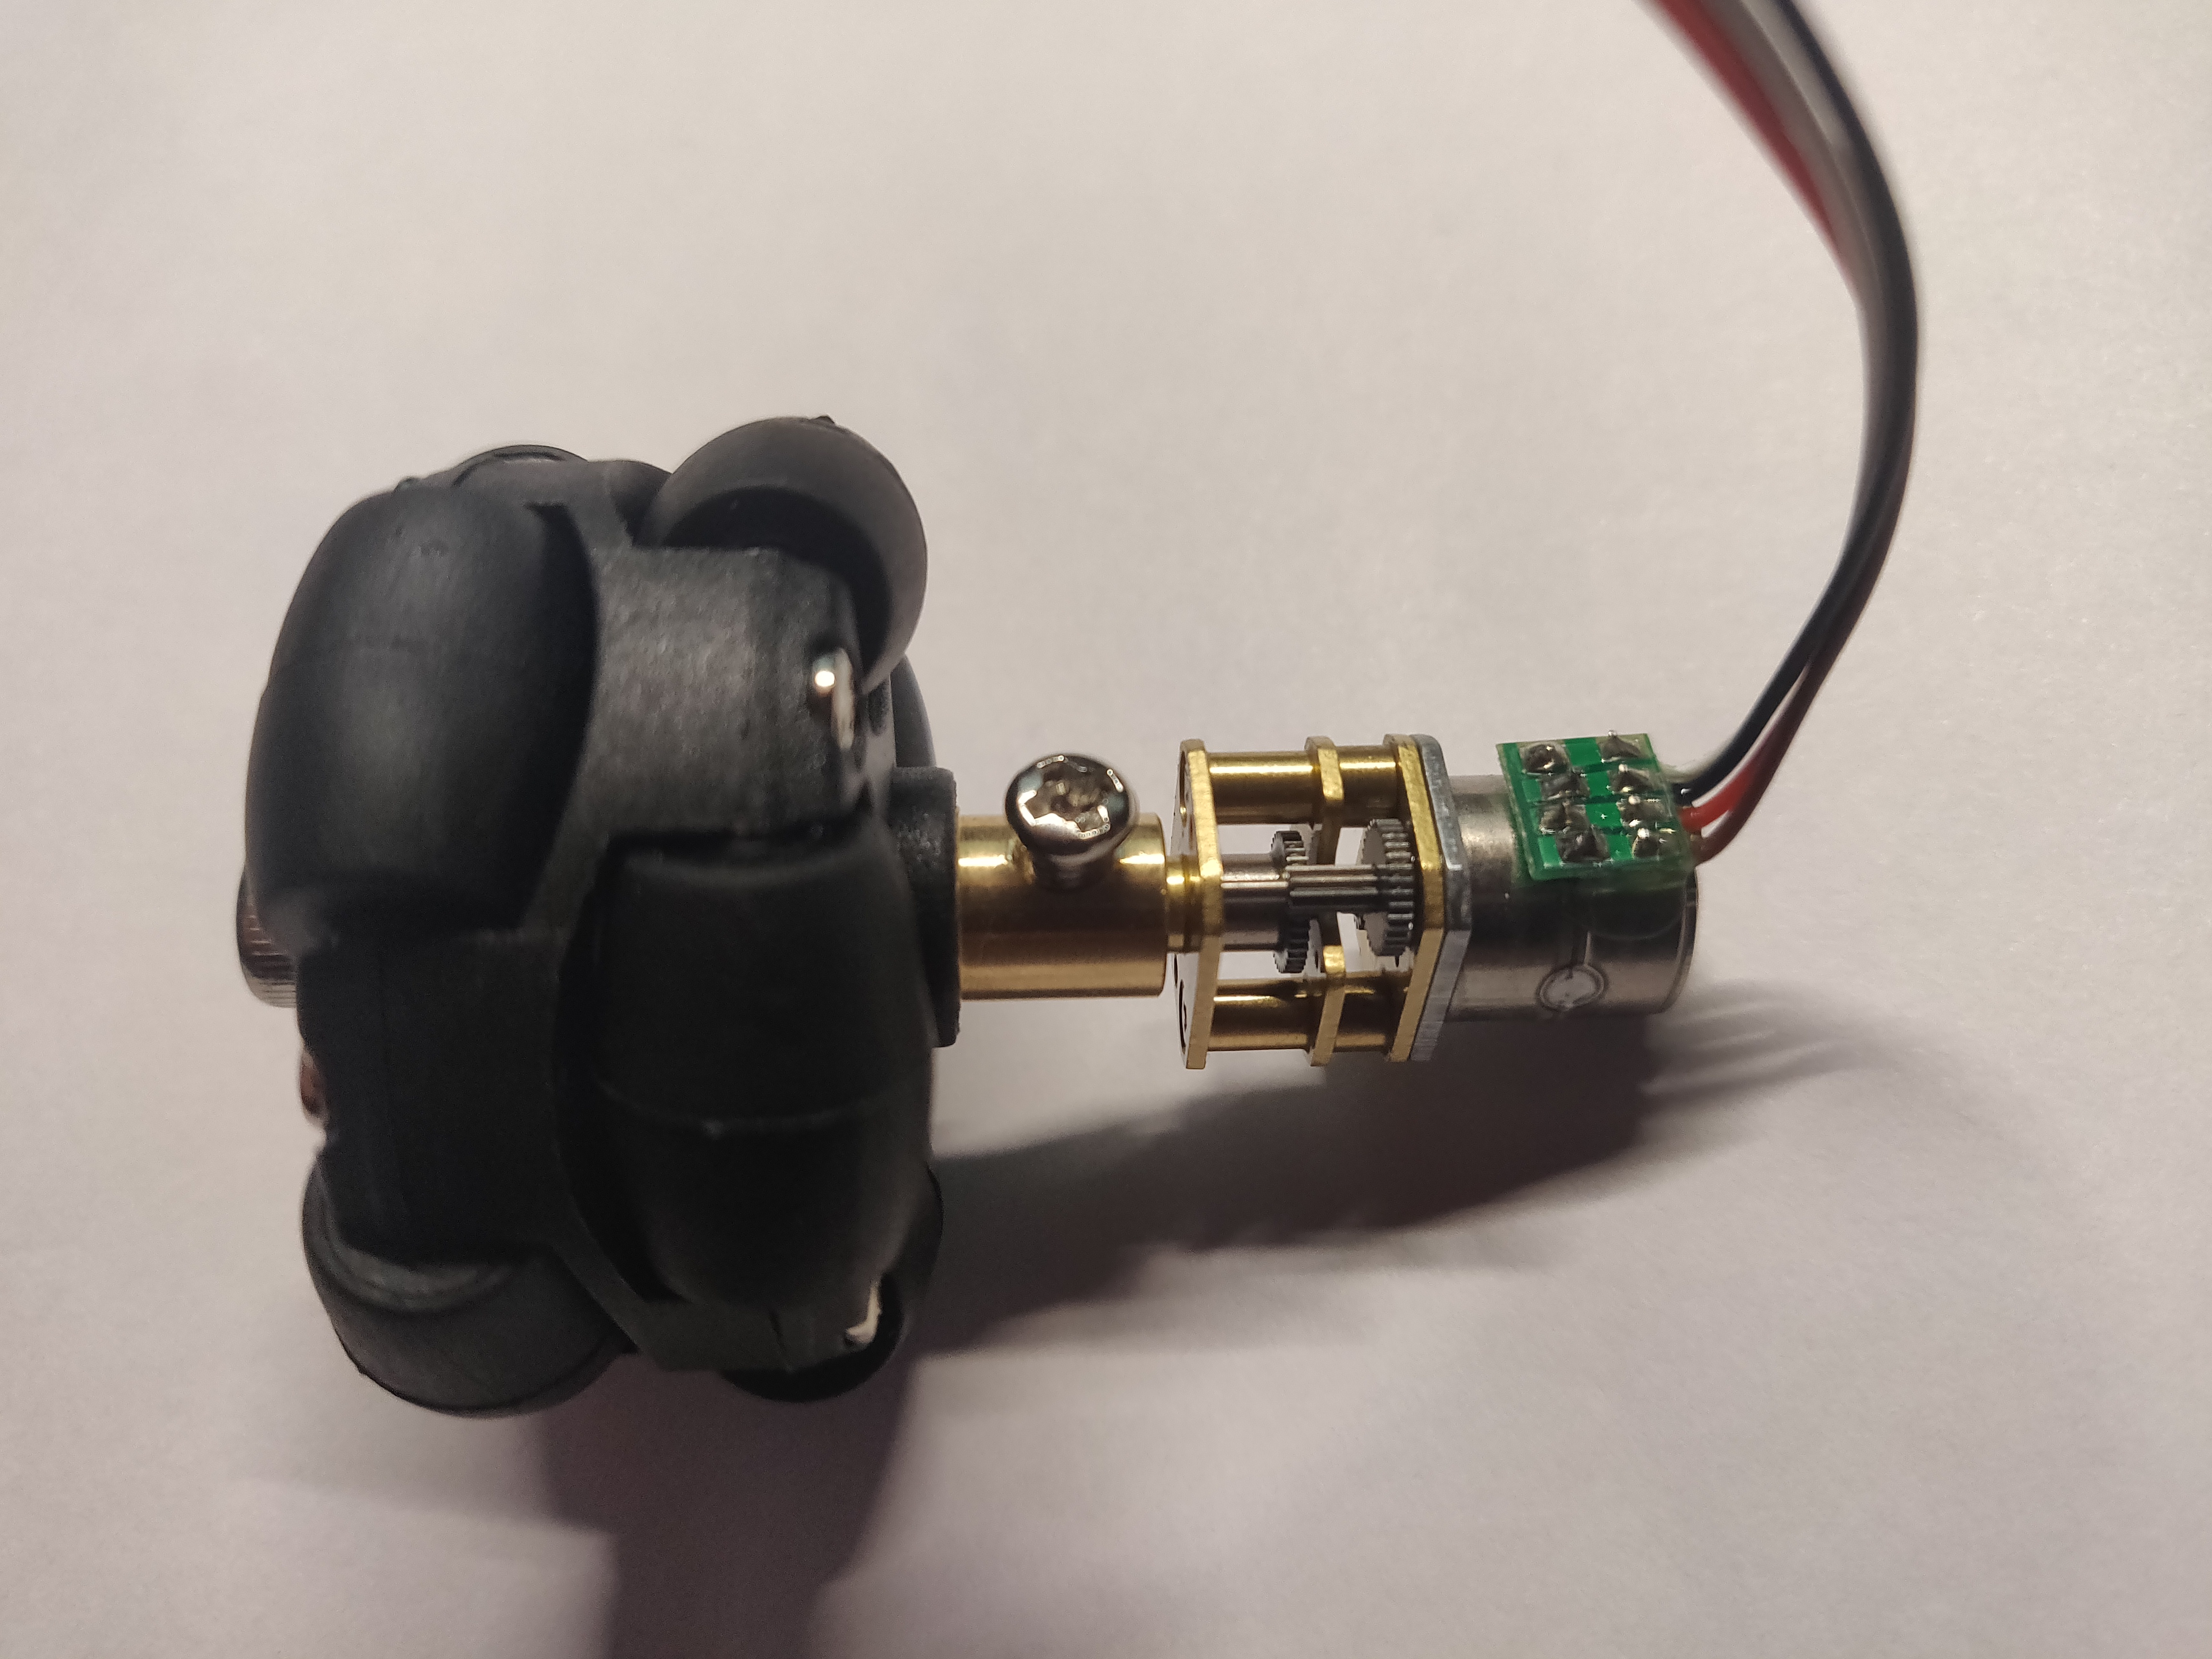
\includegraphics[height=4cm]{Motor-Step-2.jpg}
    \caption{微型步进电机(小)}
    \label{fig:Motor-Step-2}
  \end{minipage}\hfill
  \begin{minipage}{0.31\textwidth}
    \centering
    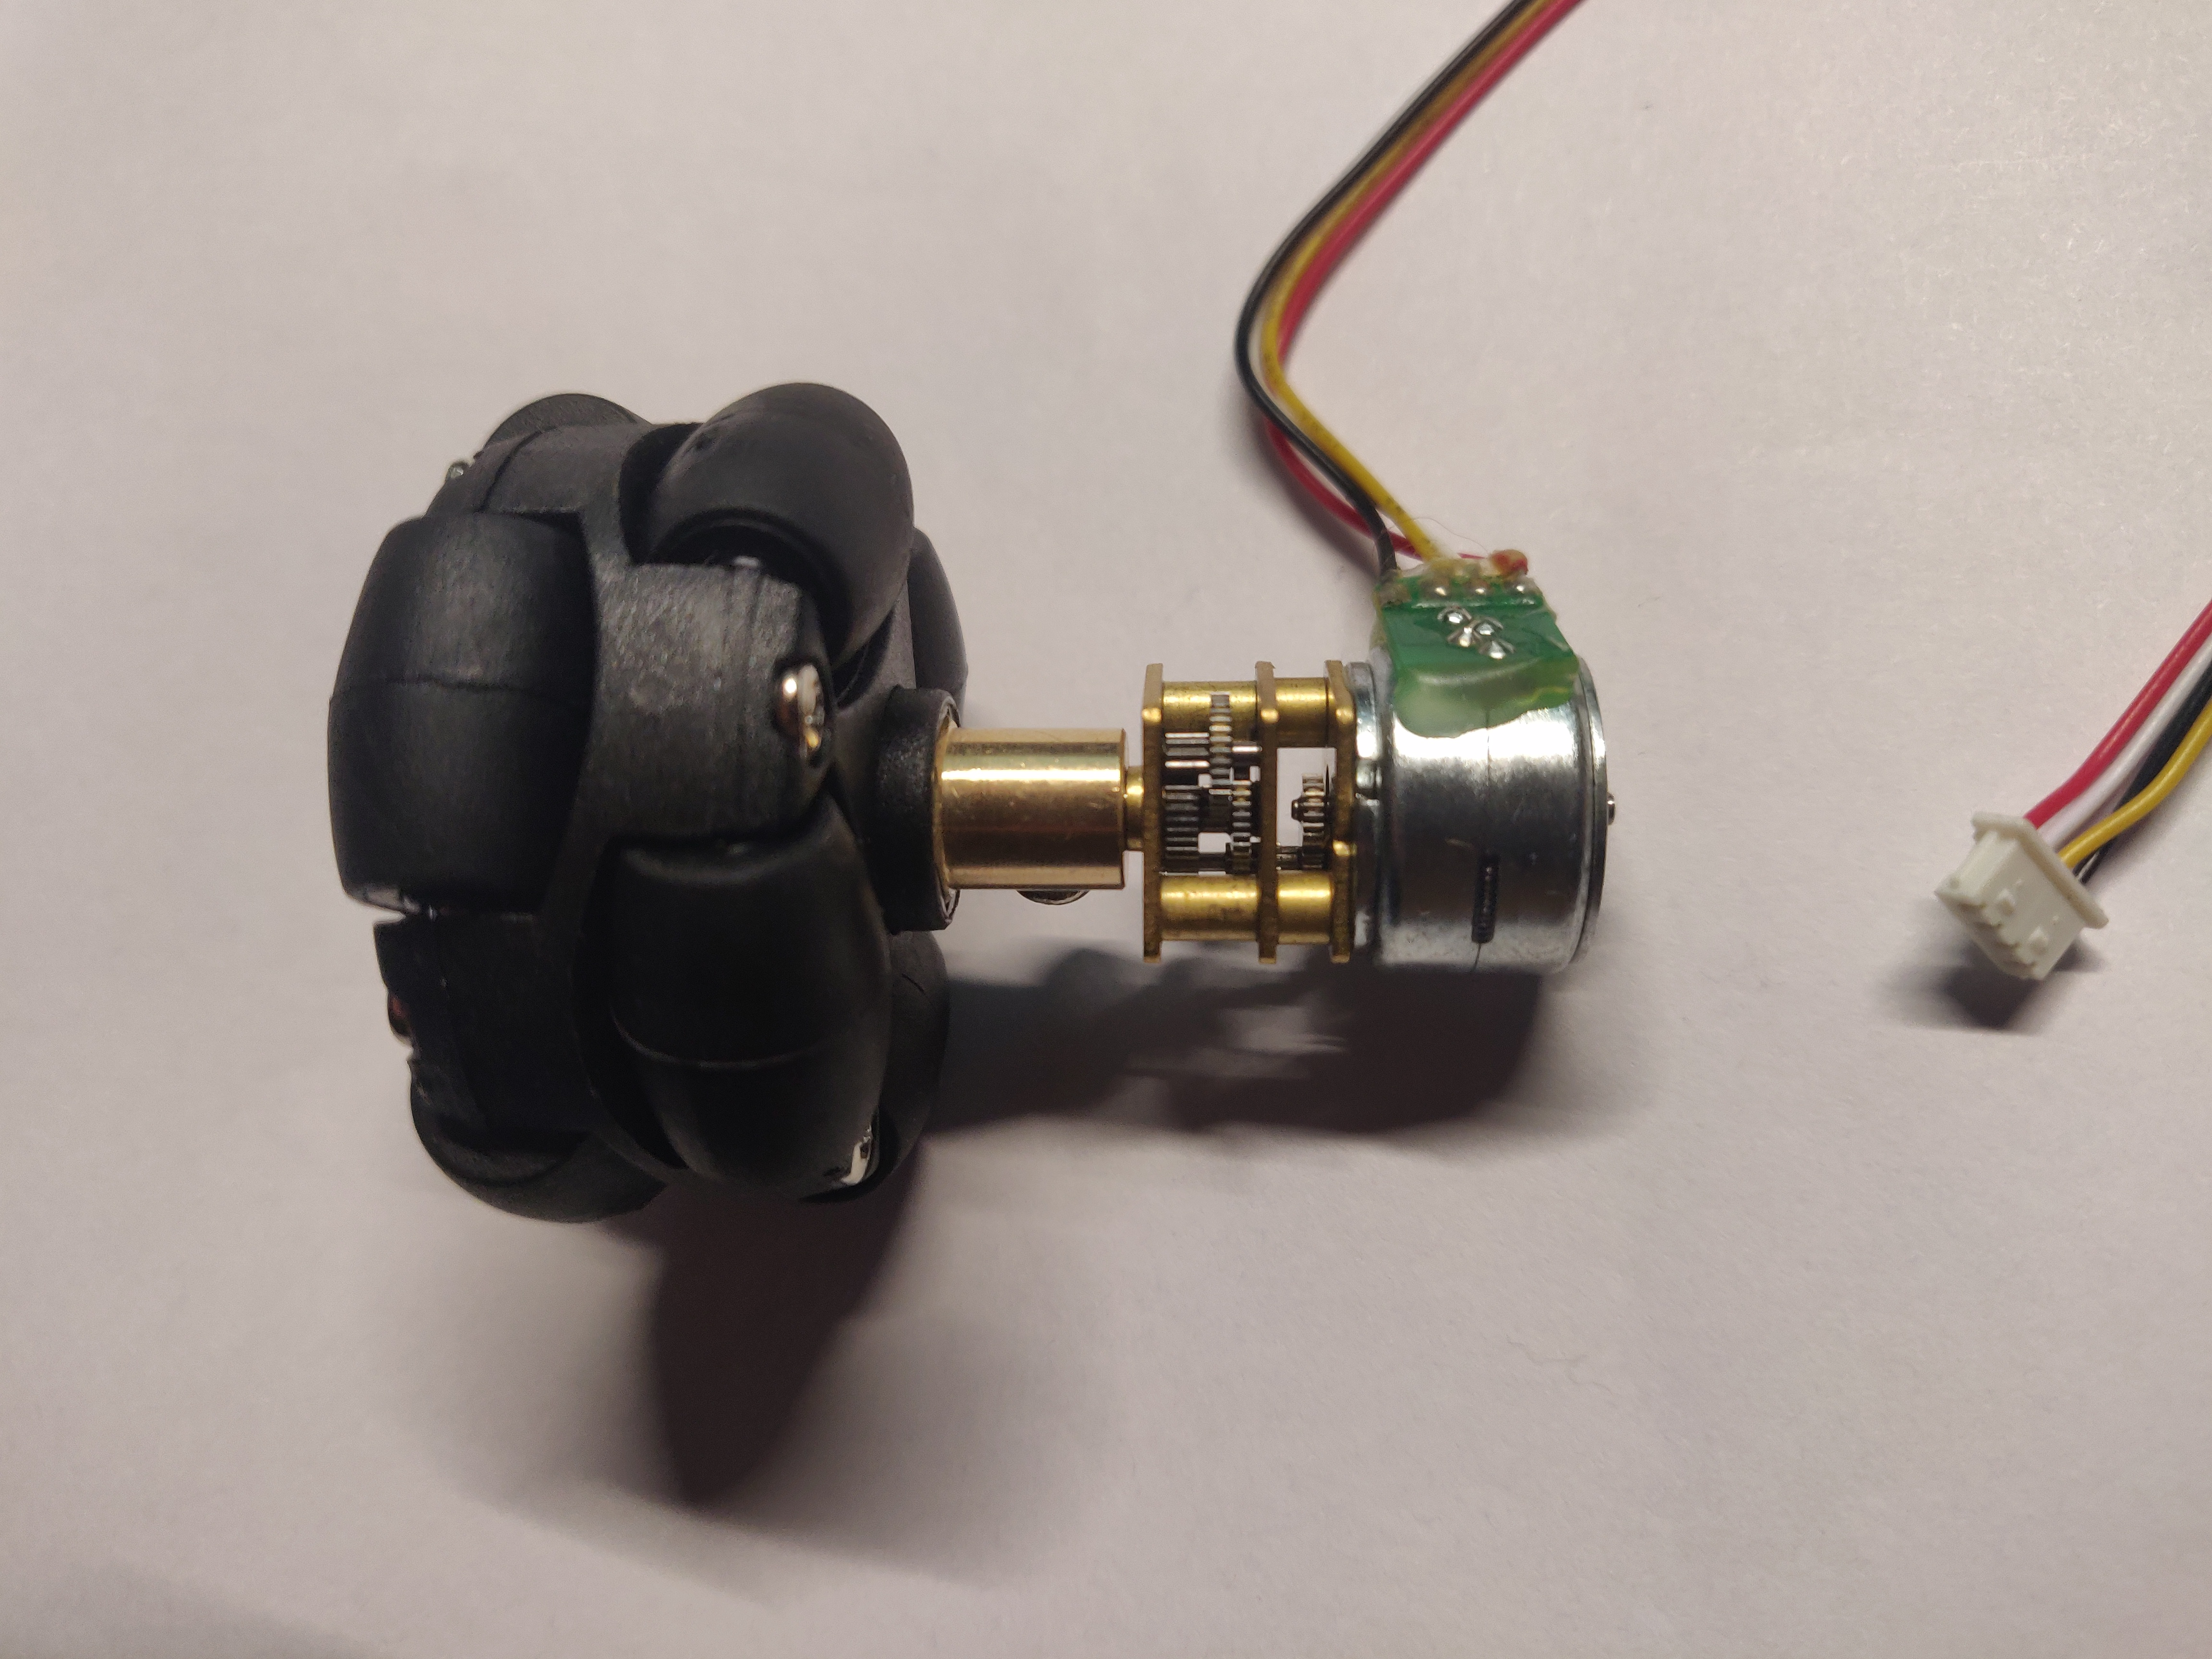
\includegraphics[height=4cm]{Motor-Step-3.jpg}
    \caption{微型步进电机(大)}
    \label{fig:Motor-Step-3}
  \end{minipage}
\end{figure}


%%% 其它部分
\backmatter

%% 本科生要这几个索引,研究生不要。选择性留下。
% 插图索引
\listoffigures
% 表格索引
\listoftables
% 公式索引
\listofequations


%% 参考文献
% 只能选择一种参考文献格式
\bibliographystyle{thuthesis-numeric}      % 顺序编码制
% \bibliographystyle{thuthesis-author-year}  % 著者-出版年制
% \bibliographystyle{thuthesis-bachelor}     % 本科生参考文献的著录格式
\bibliography{ref/refs}


%% 致谢
% 如果使用声明扫描页,将可选参数指定为扫描后的 PDF 文件名,例如:
% \begin{acknowledgement}[scan-statement.pdf]
\begin{acknowledgement}
  感谢导师钟海旺老师对本人的精心指导。

  % 感谢团队里的其他同学,目前来看,无论是作为工科的算法还是人机交互方向测试平台,这一平台有着广阔前景和无限可能,我也发现这一平台的有趣之处,希望未来能一起将这一项目继续做下去。

  感谢清华大学未来实验室的米海鹏老师及其他老师同学们,未来实验室拓展了我在集群交互领域的视野。

  感谢清华大学天空工场学生兴趣团队和未来通信学生兴趣团队,我在兴趣团队中积累了各种开发能力。

  感谢我的家人和女朋友的陪伴和支持。
  
  感谢所有帮助过我的朋友们。

  % 感谢 \LaTeX 和 \thuthesis\cite{thuthesis},帮我节省了不少时间。
\end{acknowledgement}


%% 附录
\begin{appendix}
%\chapter{外文资料原文}
\label{cha:engorg}

\title{The title of the English paper}

\textbf{Abstract:} As one of the most widely used techniques in operations
research, \emph{ mathematical programming} is defined as a means of maximizing a
quantity known as \emph{bjective function}, subject to a set of constraints
represented by equations and inequalities. Some known subtopics of mathematical
programming are linear programming, nonlinear programming, multiobjective
programming, goal programming, dynamic programming, and multilevel
programming$^{[1]}$.

It is impossible to cover in a single chapter every concept of mathematical
programming. This chapter introduces only the basic concepts and techniques of
mathematical programming such that readers gain an understanding of them
throughout the book$^{[2,3]}$.


\section{Single-Objective Programming}
The general form of single-objective programming (SOP) is written
as follows,
\begin{equation*} % 如果附录中的公式不想让它出现在公式索引中,那就请
                             % 用 equation*
\left\{\begin{array}{l}
\max \,\,f(x)\\[0.1 cm]
\mbox{subject to:} \\ [0.1 cm]
\qquad g_j(x)\le 0,\quad j=1,2,\cdots,p
\end{array}\right.
\end{equation*}
which maximizes a real-valued function $f$ of
$x=(x_1,x_2,\cdots,x_n)$ subject to a set of constraints.

\newcommand\Real{\mathbf{R}}
\newtheorem{mpdef}{Definition}[chapter]
\begin{mpdef}
In SOP, we call $x$ a decision vector, and
$x_1,x_2,\cdots,x_n$ decision variables. The function
$f$ is called the objective function. The set
\begin{equation*}
S=\left\{x\in\Real^n\bigm|g_j(x)\le 0,\,j=1,2,\cdots,p\right\}
\end{equation*}
is called the feasible set. An element $x$ in $S$ is called a
feasible solution.
\end{mpdef}

\newtheorem{mpdefop}[mpdef]{Definition}
\begin{mpdefop}
A feasible solution $x^*$ is called the optimal
solution of SOP if and only if
\begin{equation}
f(x^*)\ge f(x)
\end{equation}
for any feasible solution $x$.
\end{mpdefop}

One of the outstanding contributions to mathematical programming was known as
the Kuhn-Tucker conditions\ref{eq:ktc}. In order to introduce them, let us give
some definitions. An inequality constraint $g_j(x)\le 0$ is said to be active at
a point $x^*$ if $g_j(x^*)=0$. A point $x^*$ satisfying $g_j(x^*)\le 0$ is said
to be regular if the gradient vectors $\nabla g_j(x)$ of all active constraints
are linearly independent.

Let $x^*$ be a regular point of the constraints of SOP and assume that all the
functions $f(x)$ and $g_j(x),j=1,2,\cdots,p$ are differentiable. If $x^*$ is a
local optimal solution, then there exist Lagrange multipliers
$\lambda_j,j=1,2,\cdots,p$ such that the following Kuhn-Tucker conditions hold,
\begin{equation}
\label{eq:ktc}
\left\{\begin{array}{l}
    \nabla f(x^*)-\sum\limits_{j=1}^p\lambda_j\nabla g_j(x^*)=0\\[0.3cm]
    \lambda_jg_j(x^*)=0,\quad j=1,2,\cdots,p\\[0.2cm]
    \lambda_j\ge 0,\quad j=1,2,\cdots,p.
\end{array}\right.
\end{equation}
If all the functions $f(x)$ and $g_j(x),j=1,2,\cdots,p$ are convex and
differentiable, and the point $x^*$ satisfies the Kuhn-Tucker conditions
(\ref{eq:ktc}), then it has been proved that the point $x^*$ is a global optimal
solution of SOP.

\subsection{Linear Programming}
\label{sec:lp}

If the functions $f(x),g_j(x),j=1,2,\cdots,p$ are all linear, then SOP is called
a {\em linear programming}.

The feasible set of linear is always convex. A point $x$ is called an extreme
point of convex set $S$ if $x\in S$ and $x$ cannot be expressed as a convex
combination of two points in $S$. It has been shown that the optimal solution to
linear programming corresponds to an extreme point of its feasible set provided
that the feasible set $S$ is bounded. This fact is the basis of the {\em simplex
  algorithm} which was developed by Dantzig as a very efficient method for
solving linear programming.
\begin{table}[ht]
\centering
  \centering
  \caption*{Table~1\hskip1em This is an example for manually numbered table, which
    would not appear in the list of tables}
  \label{tab:badtabular2}
  \begin{tabular}[c]{|m{1.5cm}|c|c|c|c|c|c|}\hline
    \multicolumn{2}{|c|}{Network Topology} & \# of nodes &
    \multicolumn{3}{c|}{\# of clients} & Server \\\hline
    GT-ITM & Waxman Transit-Stub & 600 &
    \multirow{2}{2em}{2\%}&
    \multirow{2}{2em}{10\%}&
    \multirow{2}{2em}{50\%}&
    \multirow{2}{1.2in}{Max. Connectivity}\\\cline{1-3}
    \multicolumn{2}{|c|}{Inet-2.1} & 6000 & & & &\\\hline
    \multirow{2}{1.5cm}{Xue} & Rui  & Ni &\multicolumn{4}{c|}{\multirow{2}*{\thuthesis}}\\\cline{2-3}
    & \multicolumn{2}{c|}{ABCDEF} &\multicolumn{4}{c|}{} \\\hline
\end{tabular}
\end{table}

Roughly speaking, the simplex algorithm examines only the extreme points of the
feasible set, rather than all feasible points. At first, the simplex algorithm
selects an extreme point as the initial point. The successive extreme point is
selected so as to improve the objective function value. The procedure is
repeated until no improvement in objective function value can be made. The last
extreme point is the optimal solution.

\subsection{Nonlinear Programming}

If at least one of the functions $f(x),g_j(x),j=1,2,\cdots,p$ is nonlinear, then
SOP is called a {\em nonlinear programming}.

A large number of classical optimization methods have been developed to treat
special-structural nonlinear programming based on the mathematical theory
concerned with analyzing the structure of problems.
\begin{figure}[h]
  \centering
  
\includegraphics{thu-lib-logo.pdf}
  \caption*{Figure~1\quad This is an example for manually numbered figure,
    which would not appear in the list of figures}
  \label{tab:badfigure2}
\end{figure}

Now we consider a nonlinear programming which is confronted solely with
maximizing a real-valued function with domain $\Real^n$.  Whether derivatives are
available or not, the usual strategy is first to select a point in $\Real^n$ which
is thought to be the most likely place where the maximum exists. If there is no
information available on which to base such a selection, a point is chosen at
random. From this first point an attempt is made to construct a sequence of
points, each of which yields an improved objective function value over its
predecessor. The next point to be added to the sequence is chosen by analyzing
the behavior of the function at the previous points. This construction continues
until some termination criterion is met. Methods based upon this strategy are
called {\em ascent methods}, which can be classified as {\em direct methods},
{\em gradient methods}, and {\em Hessian methods} according to the information
about the behavior of objective function $f$. Direct methods require only that
the function can be evaluated at each point. Gradient methods require the
evaluation of first derivatives of $f$. Hessian methods require the evaluation
of second derivatives. In fact, there is no superior method for all
problems. The efficiency of a method is very much dependent upon the objective
function.

\subsection{Integer Programming}

{\em Integer programming} is a special mathematical programming in which all of
the variables are assumed to be only integer values. When there are not only
integer variables but also conventional continuous variables, we call it {\em
  mixed integer programming}. If all the variables are assumed either 0 or 1,
then the problem is termed a {\em zero-one programming}. Although integer
programming can be solved by an {\em exhaustive enumeration} theoretically, it
is impractical to solve realistically sized integer programming problems. The
most successful algorithm so far found to solve integer programming is called
the {\em branch-and-bound enumeration} developed by Balas (1965) and Dakin
(1965). The other technique to integer programming is the {\em cutting plane
  method} developed by Gomory (1959).

\hfill\textit{Uncertain Programming\/}\quad(\textsl{BaoDing Liu, 2006.2})

\section*{References}
\noindent{\itshape NOTE: These references are only for demonstration. They are
  not real citations in the original text.}

\begin{translationbib}
\item Donald E. Knuth. The \TeX book. Addison-Wesley, 1984. ISBN: 0-201-13448-9
\item Paul W. Abrahams, Karl Berry and Kathryn A. Hargreaves. \TeX\ for the
  Impatient. Addison-Wesley, 1990. ISBN: 0-201-51375-7
\item David Salomon. The advanced \TeX book.  New York : Springer, 1995. ISBN:0-387-94556-3
\end{translationbib}

\chapter{外文资料的调研阅读报告或书面翻译}

\title{英文资料的中文标题}

{\heiti 摘要:} 本章为外文资料翻译内容。如果有摘要可以直接写上来,这部分好像没有
明确的规定。

\section{单目标规划}
北冥有鱼,其名为鲲。鲲之大,不知其几千里也。化而为鸟,其名为鹏。鹏之背,不知其几
千里也。怒而飞,其翼若垂天之云。是鸟也,海运则将徙于南冥。南冥者,天池也。
\begin{equation}\tag*{(123)}
 p(y|\mathbf{x}) = \frac{p(\mathbf{x},y)}{p(\mathbf{x})}=
\frac{p(\mathbf{x}|y)p(y)}{p(\mathbf{x})}
\end{equation}

吾生也有涯,而知也无涯。以有涯随无涯,殆已!已而为知者,殆而已矣!为善无近名,为
恶无近刑,缘督以为经,可以保身,可以全生,可以养亲,可以尽年。

\subsection{线性规划}
庖丁为文惠君解牛,手之所触,肩之所倚,足之所履,膝之所倚,砉然响然,奏刀騞然,莫
不中音,合于桑林之舞,乃中经首之会。
\begin{table}[ht]
\centering
  \centering
  \caption*{表~1\hskip1em 这是手动编号但不出现在索引中的一个表格例子}
  \label{tab:badtabular3}
  \begin{tabular}[c]{|m{1.5cm}|c|c|c|c|c|c|}\hline
    \multicolumn{2}{|c|}{Network Topology} & \# of nodes &
    \multicolumn{3}{c|}{\# of clients} & Server \\\hline
    GT-ITM & Waxman Transit-Stub & 600 &
    \multirow{2}{2em}{2\%}&
    \multirow{2}{2em}{10\%}&
    \multirow{2}{2em}{50\%}&
    \multirow{2}{1.2in}{Max. Connectivity}\\\cline{1-3}
    \multicolumn{2}{|c|}{Inet-2.1} & 6000 & & & &\\\hline
    \multirow{2}{1.5cm}{Xue} & Rui  & Ni &\multicolumn{4}{c|}{\multirow{2}*{\thuthesis}}\\\cline{2-3}
    & \multicolumn{2}{c|}{ABCDEF} &\multicolumn{4}{c|}{} \\\hline
\end{tabular}
\end{table}

文惠君曰:“嘻,善哉!技盖至此乎?”庖丁释刀对曰:“臣之所好者道也,进乎技矣。始臣之
解牛之时,所见无非全牛者;三年之后,未尝见全牛也;方今之时,臣以神遇而不以目视,
官知止而神欲行。依乎天理,批大郤,导大窾,因其固然。技经肯綮之未尝,而况大坬乎!
良庖岁更刀,割也;族庖月更刀,折也;今臣之刀十九年矣,所解数千牛矣,而刀刃若新发
于硎。彼节者有间而刀刃者无厚,以无厚入有间,恢恢乎其于游刃必有余地矣。是以十九年
而刀刃若新发于硎。虽然,每至于族,吾见其难为,怵然为戒,视为止,行为迟,动刀甚微,
謋然已解,如土委地。提刀而立,为之而四顾,为之踌躇满志,善刀而藏之。”

文惠君曰:“善哉!吾闻庖丁之言,得养生焉。”


\subsection{非线性规划}
孔子与柳下季为友,柳下季之弟名曰盗跖。盗跖从卒九千人,横行天下,侵暴诸侯。穴室枢
户,驱人牛马,取人妇女。贪得忘亲,不顾父母兄弟,不祭先祖。所过之邑,大国守城,小
国入保,万民苦之。孔子谓柳下季曰:“夫为人父者,必能诏其子;为人兄者,必能教其弟。
若父不能诏其子,兄不能教其弟,则无贵父子兄弟之亲矣。今先生,世之才士也,弟为盗
跖,为天下害,而弗能教也,丘窃为先生羞之。丘请为先生往说之。”
\begin{figure}[h]
  \centering
  
\includegraphics{thu-whole-logo.pdf}
  \caption*{图~1\hskip1em 这是手动编号但不出现索引中的图片的例子}
  \label{tab:badfigure3}
\end{figure}

柳下季曰:“先生言为人父者必能诏其子,为人兄者必能教其弟,若子不听父之诏,弟不受
兄之教,虽今先生之辩,将奈之何哉?且跖之为人也,心如涌泉,意如飘风,强足以距敌,
辩足以饰非。顺其心则喜,逆其心则怒,易辱人以言。先生必无往。”

孔子不听,颜回为驭,子贡为右,往见盗跖。

\subsection{整数规划}
盗跖乃方休卒徒大山之阳,脍人肝而餔之。孔子下车而前,见谒者曰:“鲁人孔丘,闻将军
高义,敬再拜谒者。”谒者入通。盗跖闻之大怒,目如明星,发上指冠,曰:“此夫鲁国之
巧伪人孔丘非邪?为我告之:尔作言造语,妄称文、武,冠枝木之冠,带死牛之胁,多辞缪
说,不耕而食,不织而衣,摇唇鼓舌,擅生是非,以迷天下之主,使天下学士不反其本,妄
作孝弟,而侥幸于封侯富贵者也。子之罪大极重,疾走归!不然,我将以子肝益昼餔之膳。”


\chapter{其它附录}
前面两个附录主要是给本科生做例子。其它附录的内容可以放到这里,当然如果你愿意,可
以把这部分也放到独立的文件中,然后将其 \cs{input} 到主文件中。

\end{appendix}

%% 个人简历
%\begin{resume}

  \resumeitem{个人简历}

  xxxx 年 xx 月 xx 日出生于 xx 省 xx 县。

  xxxx 年 9 月考入 xx 大学 xx 系 xx 专业,xxxx 年 7 月本科毕业并获得 xx 学士学位。

  xxxx 年 9 月免试进入 xx 大学 xx 系攻读 xx 学位至今。

  \researchitem{发表的学术论文} % 发表的和录用的合在一起

  % 1. 已经刊载的学术论文(本人是第一作者,或者导师为第一作者本人是第二作者)
  \begin{publications}
    \item Yang Y, Ren T L, Zhang L T, et al. Miniature microphone with silicon-
      based ferroelectric thin films. Integrated Ferroelectrics, 2003,
      52:229-235. (SCI 收录, 检索号:758FZ.)
    \item 杨轶, 张宁欣, 任天令, 等. 硅基铁电微声学器件中薄膜残余应力的研究. 中国机
      械工程, 2005, 16(14):1289-1291. (EI 收录, 检索号:0534931 2907.)
    \item 杨轶, 张宁欣, 任天令, 等. 集成铁电器件中的关键工艺研究. 仪器仪表学报,
      2003, 24(S4):192-193. (EI 源刊.)
  \end{publications}

  % 2. 尚未刊载,但已经接到正式录用函的学术论文(本人为第一作者,或者
  %    导师为第一作者本人是第二作者)。
  \begin{publications}[before=\publicationskip,after=\publicationskip]
    \item Yang Y, Ren T L, Zhu Y P, et al. PMUTs for handwriting recognition. In
      press. (已被 Integrated Ferroelectrics 录用. SCI 源刊.)
  \end{publications}

  % 3. 其他学术论文。可列出除上述两种情况以外的其他学术论文,但必须是
  %    已经刊载或者收到正式录用函的论文。
  \begin{publications}
    \item Wu X M, Yang Y, Cai J, et al. Measurements of ferroelectric MEMS
      microphones. Integrated Ferroelectrics, 2005, 69:417-429. (SCI 收录, 检索号
      :896KM)
    \item 贾泽, 杨轶, 陈兢, 等. 用于压电和电容微麦克风的体硅腐蚀相关研究. 压电与声
      光, 2006, 28(1):117-119. (EI 收录, 检索号:06129773469)
    \item 伍晓明, 杨轶, 张宁欣, 等. 基于MEMS技术的集成铁电硅微麦克风. 中国集成电路,
      2003, 53:59-61.
  \end{publications}

  \researchitem{研究成果} % 有就写,没有就删除
  \begin{achievements}
    \item 任天令, 杨轶, 朱一平, 等. 硅基铁电微声学传感器畴极化区域控制和电极连接的
      方法: 中国, CN1602118A. (中国专利公开号)
    \item Ren T L, Yang Y, Zhu Y P, et al. Piezoelectric micro acoustic sensor
      based on ferroelectric materials: USA, No.11/215, 102. (美国发明专利申请号)
  \end{achievements}

\end{resume}


%% 本科生进行格式审查是需要下面这个表格,答辩可能不需要。选择性留下。
% 综合论文训练记录表
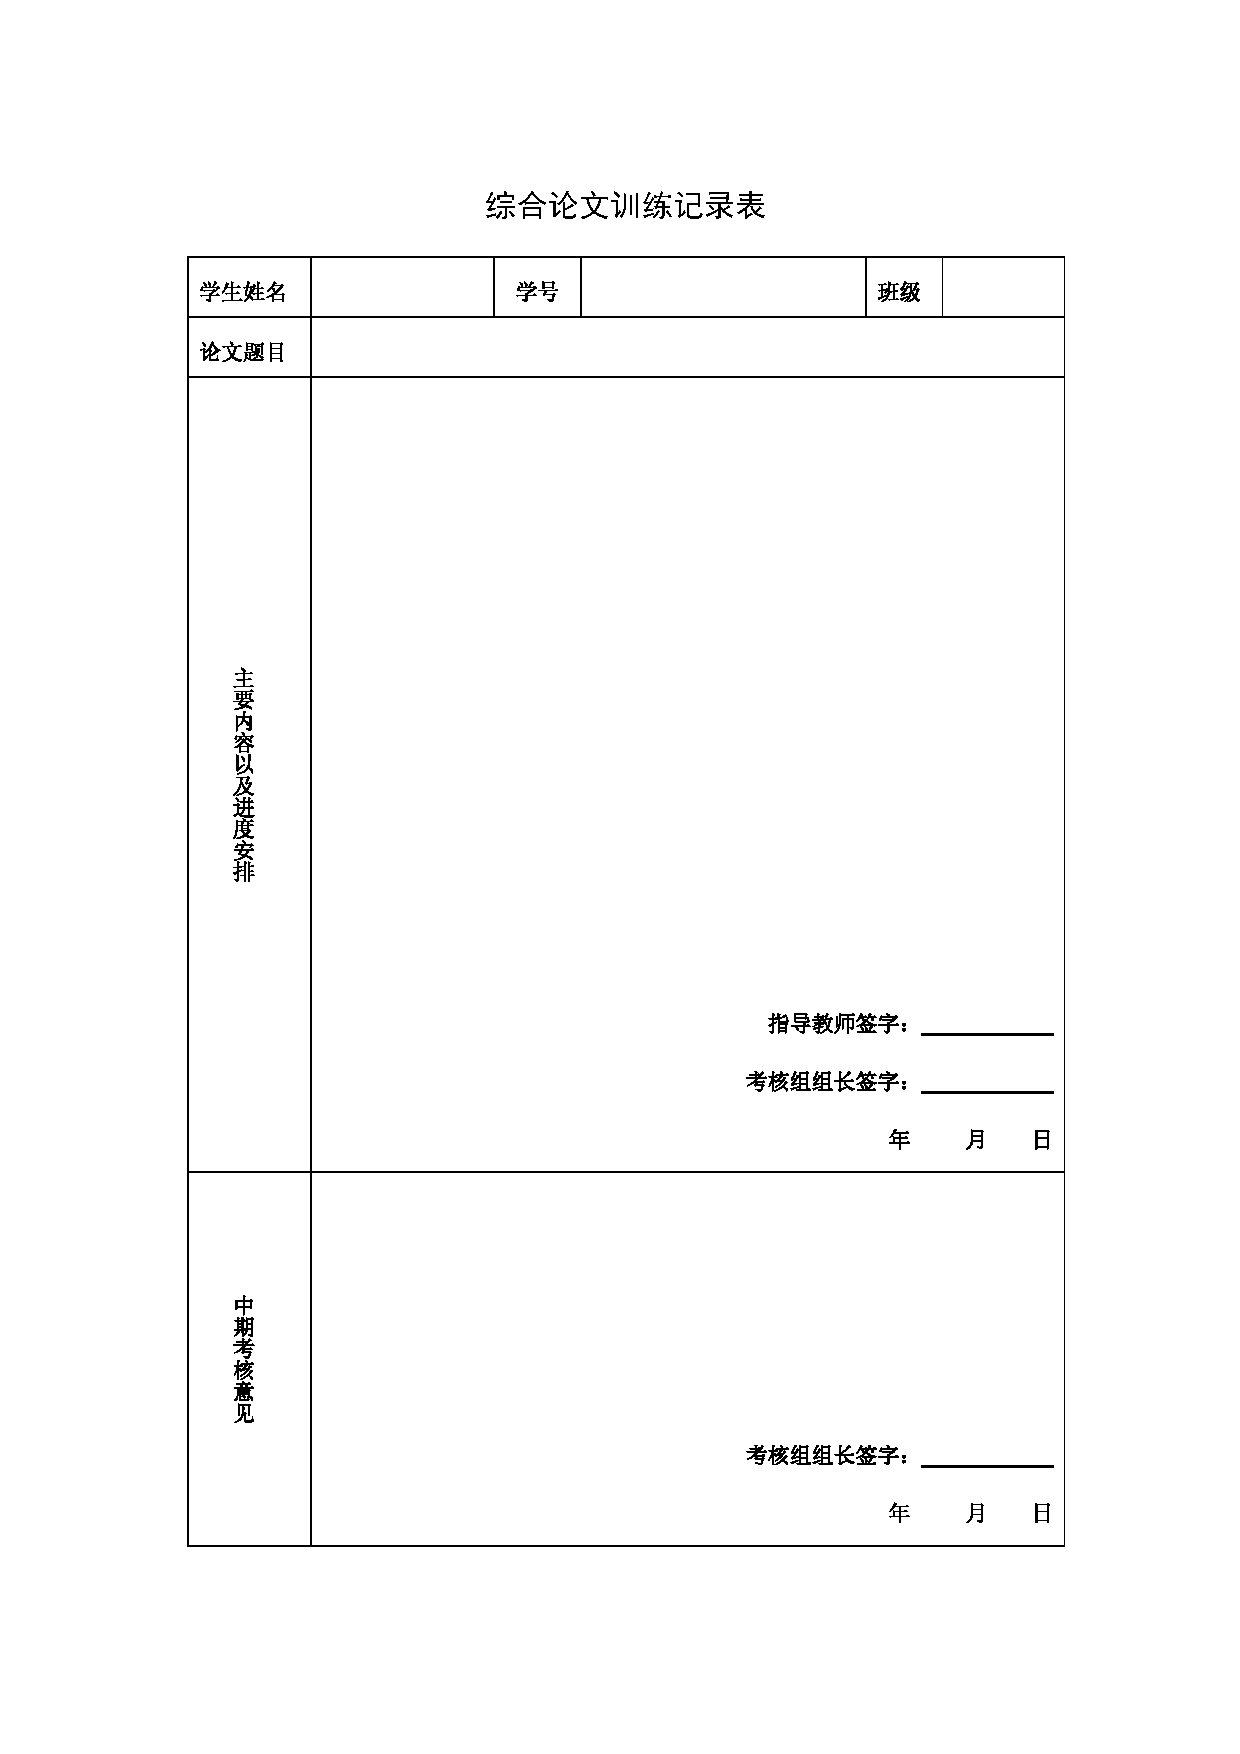
\includepdf[pages=-]{scan-record.pdf}
\end{document}
